% Este simbolo es para comentar
% Definicion de tipo de documento y tamaño de letra
\documentclass[11pt]{report}
%%%%%%%%%%%%%%%%%%%%%%%%%
%%%%%%%%%%%%%%%%%
%%%%%%%%%%%%%%%%%%%%% Preambulo
%%%%%%%%%%%%%%%
%%%%%%%%%%%%% Paquetes a utilizar en el documento

\usepackage[T1]{fontenc}
\usepackage[utf8]{inputenc}
\usepackage[spanish]{babel}
\usepackage{times}
\usepackage{tocbibind} % Para incluir la bibliografía en el índice
\usepackage{tikz}
\usetikzlibrary{shapes, arrows, positioning}
\usepackage{listings}
\usepackage{tabularx}
\usepackage{colortbl}
\usepackage{cite}
\usepackage{xcolor}
\usepackage{geometry} % Allows the configuration of document margins
\geometry{papersize={216mm,330mm}, hmargin={3cm,0.8in}, height=10.5in}
\usepackage{graphicx, caption}
\usepackage{csquotes}
\usepackage{setspace}
\usepackage{float}
\usepackage{tcolorbox}
\usepackage{fancyhdr} % http://mirror.easyname.at/ctan/macros/latex/contrib/fancyhdr/fancyhdr.pdf
\usepackage{titlesec}
\usepackage{hyperref}
\usepackage{amsmath}


% Configuración de hyperref
\hypersetup{
	colorlinks,
	citecolor=black,
	filecolor=black,
	linkcolor=black,
	urlcolor=black
}

%%%%%%
% Paquete para manejar el encabezado y pie de página
%%%%%%
\pagestyle{fancy} 
\fancyhead[L]{\rightmark}
\setlength\headheight{50pt}
\fancyhead[R]{\raisebox{-0.5\height}{
\includegraphics[width=2.2cm]{Imagenes/unican.png}}}
\fancyfoot{}
\fancyfoot[L]{\raisebox{-0.5\height}{
\includegraphics[width=2.2cm]{Imagenes/facitecLogo1.jpg}}}
\fancyfoot[R]{\thepage}

\linespread{1.25} % Interlineado
%\setlength{\parskip}{1em} % Espaciado de párrafo

% Configuración de títulos
\titleformat{\chapter}
{\normalfont\Huge\bfseries}{\thechapter}{1em}{}

\lstset{
	language=Bash,
	basicstyle=\ttfamily,
	numbers=left,
	numberstyle=\tiny,
	stepnumber=1,
	numbersep=5pt,
	backgroundcolor=\color{white},
	frame=single,
	captionpos=b,
	breaklines=true,
	breakatwhitespace=false,
	tabsize=4
}

\begin{document}
	
	% Información del documento
	\title{Sistema Operativo}
	\author{Luis Torres}
	\date{Canindeyú, Paraguay, 2024}
	
	% CARATULA
	\begin{titlepage}
		\begin{center}
			
\includegraphics[width=0.3\linewidth]{Imagenes/facitecLogo1.jpg}
			\vspace{15pt}
			
			{\scshape\LARGE\textbf{Facultad de Ciencias y Tecnología}\\}
			{\Large\itshape Universidad Nacional de Canindeyú\\}
			
			\vspace{1cm}
			{\huge\scshape\ \textbf{Sistema Operativo}\\}
			\vspace{1cm}
			{\huge\bfseries Material de lectura\\}
			
			{\Large\itshape Unidad 7\\}
			\vspace{1cm}
			{\Large\itshape Docente: Luis Torres\\}
			
			\vfill
			\vfill
			
			% Parte inferior de la página
			{\large Canindeyú, Paraguay, 2024\\}
		\end{center}
	\end{titlepage}
	
	\newpage
	
	% INDICE
	\begin{singlespacing}
		\tableofcontents
	\end{singlespacing}
	
	% Iniciando contenido
	\selectlanguage{spanish}
	
	%%%%%%%%%%%%%%%%%%%%%%%%%%%%%%%%%%%
	%%%%%%%%%% CONTENIDO
	%%%%%%%%%%%%%%
	%\chapter{Introducción a los sistemas operativos}
\section{
Introducción
}
Es necesario comprender que la actividad informática se centra en un elemento físico\cite{introsistema}, esto es, un equipo de cómputo.

Entre los equipos de cómputo, podemos citar:
\begin{itemize}
	\item  Computadora o PC
	\item Tablets
	\item Teléfonos inteligentes (\textit{smartphones})
\end{itemize}


Estos equipos de cómputo (en adelante, computadoras) son máquinas de origen electrónico con una o más unidades de proceso, además de otros componentes periféricos controlados por programas almacenados en su memoria. Pueden realizar una gran variedad de trabajos.

A todo componente físico de una computadora, es decir, todo aquel componente con el cual podemos interactuar físicamente, se le denomina \textit{\textbf{hardware}}.

Todo \textbf{\textit{hardware}} de una computadora necesita de información que le indique cómo funcionar. Su funcionamiento está definido por instrucciones (programas), que constituyen su soporte lógico (\textbf{\textit{software}}). 

El \textit{software} incluye tanto el sistema operativo como las aplicaciones que utilizamos para realizar tareas específicas. Sin \textit{software}, el \textit{hardware} no podría realizar ninguna operación útil.



\section{Sistema Operativo. Concepto}
Al comprender que el sistema operativo constituye un software, podemos definirlo de la siguiente forma:
\begin{tcolorbox}
	Un \textbf{Sistema Operativo }es el soporte lógico que controla el funcionamiento del equipo físico\cite{introsistema}.
\end{tcolorbox}
Dependiendo el punto de vista, podemos encontrar otras definiciones de un sistema operativo:

\begin{itemize}
	\item  \subsection{Punto de vista del USUARIO}
		\begin{tcolorbox}
			Un \textbf{Sistema Operativo }es un conjunto de programas y funciones que ocultan los detalles del hardware\cite{introsistema}, facilitando al usuario el acceso al mismo. 
	\end{tcolorbox}
	La ocultación de los detalles del hardware persigue dos objetivos:
	    \begin{itemize}
			\item \textbf{Abstracción:} El sistema operativo proporciona una interfaz simplificada que permite a los usuarios y a los desarrolladores de software interactuar con el hardware sin necesidad de conocer su funcionamiento interno. Esto se logra a través de la creación de capas de abstracción que ocultan la complejidad del hardware y presentan una interfaz más amigable y coherente.
			\item \textbf{Seguridad:} El sistema operativo implementa mecanismos de protección para asegurar que los recursos del sistema sean utilizados de manera controlada y segura. Esto incluye la gestión de permisos de acceso, la protección de la memoria, y la prevención de interferencias entre procesos, garantizando así la estabilidad y la integridad del sistema.
		\end{itemize}
	\item \subsection{Punto de vista de GESTOR DE RECURSOS}
	
		\begin{tcolorbox}
			Un \textbf{Sistema Operativo }es el administrador de recursos ofrecidos por el hardware para alcanzar un eficaz rendimiento de los mismos\cite{introsistema}.
		\end{tcolorbox}

	Los recursos fundamentales que administra son:
	
		\begin{itemize}
			\item El procesador.
			\item La memoria
			\item La entrada/salida.
			\item La información.
		\end{itemize}

	
\end{itemize}

	Basado en las definiciones mencionadas, podemos concluir que:
	
	
	\begin{tcolorbox}
		Un \textbf{Sistema Operativo }es un conjunto de programas relacionados entre si, que contribuyen a que la computadora lleve a cabo correctamente su trabajo\cite{introsistema}.
	\end{tcolorbox}
	
	Además podemos afirmar que los sistemas operativos tienen dos objetivos fundamentales:
\begin{itemize}
	\item Facilitar el trabajo al usuario.
	\item Gestionar de forma eficiente los recursos.
\end{itemize}

\section{Evolución histórica.}
A lo largo de la historia, las computadoras evolucionaron de manera espectacular, las primeras máquinas de cómputo carecían de sistema operativo y equipos de tamaño de una sala. Se describen como los sistemas operativos están estrechamente relacionados con la evolución de las computadoras.



\subsection{La primera generación (1945 a 1955): tubos de vacío}

Las primeras computadoras fueron construidas a partir de tubos de vacío, eran voluminosas y consumían mucha energía.
\begin{figure}[H]
	\centering
	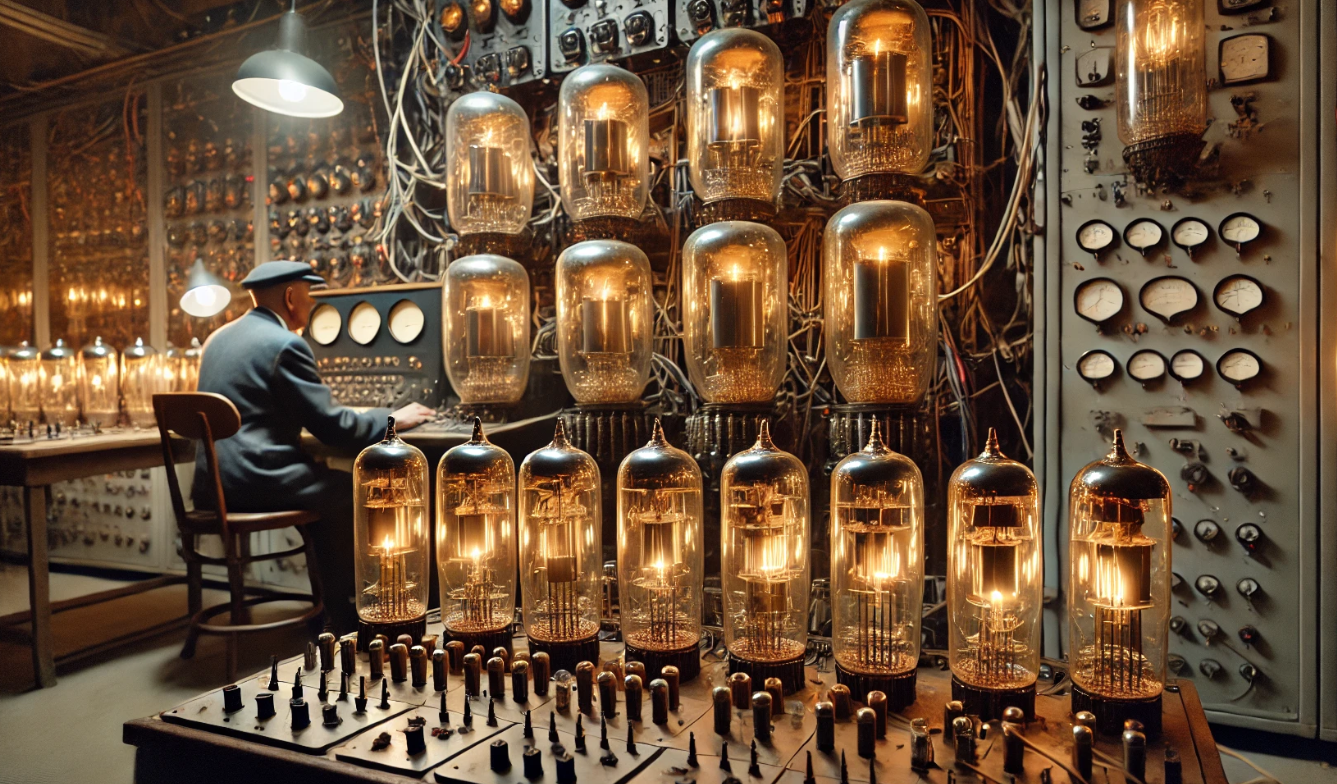
\includegraphics[width=0.5\linewidth]{Imagenes/tubos.png}
	\caption{Las primeras computadoras ocupaban salas enteras.}
	\label{fig:enter-label}
\end{figure}
En esta primera generación, no existían los lenguajes de programación de alto nivel ni los sistemas operativos tal como los conocemos hoy en día. La ejecución de tareas era rudimentaria; mediante tarjetas perforadas, los ingenieros transmitían las instrucciones a las máquinas.
\begin{figure}[H]
	\centering
	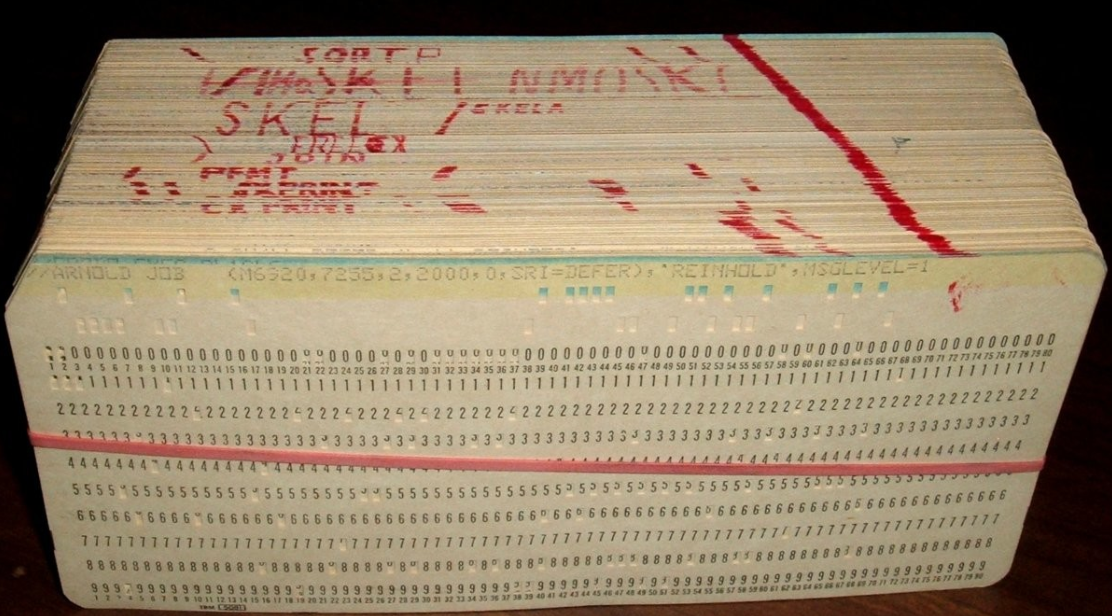
\includegraphics[width=0.6\linewidth]{Imagenes/tarjetas.png}
	\caption{Una pila de tarjetas perforadas, que podían contener un conjunto de instrucciones.}
	\label{fig:enter-label}
\end{figure}

\subsection{La segunda generación (1955 a 1965): los transistores}

La llegada de los transistores a mediados de la década de los 50 lo cambió todo. Este evento permitió la construcción de computadoras más pequeñas, además de ser mucho más eficientes, los transistores consumían mucho menos energía. Los transistores aumentaron la velocidad de procesamiento, permitiendo realizar operaciones mucho más rápidas, finalmente los transistores popularizaron los equipos de cómputo al reducir el costo de fabricación.

\begin{figure}[H]
	\centering
	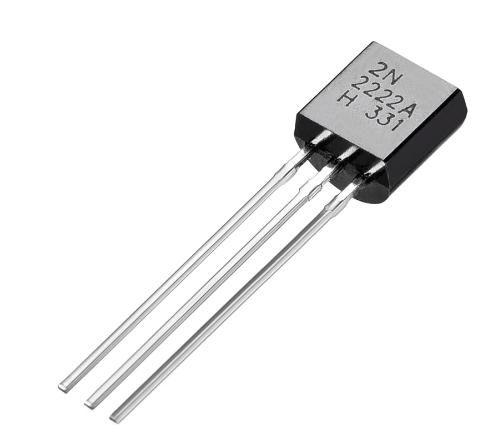
\includegraphics[width=0.4\linewidth]{Imagenes/transistor.png}
	\caption{Los transistores permitieron la fabricación de computadoras más compactas y portátiles.}
	\label{fig:enter-label}
\end{figure}

En 1957 surge FORTRAN (FORmula TRANslation), uno de los primeros lenguajes de programación de alto nivel desarrollado por IBM.

FORTRAN revolucionó la programación, haciendo más accesible el uso de computadoras para científicos e ingenieros y estableciendo estándares que influenciarían futuros lenguajes de programación.

\begin{figure}[H]
	\centering
	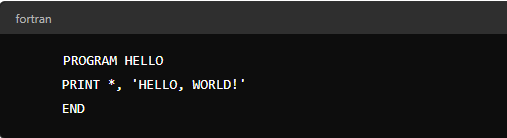
\includegraphics[width=0.8\linewidth]{Imagenes/fortran.png}
	\caption{Ejemplo de programa escrito con FORTRAN.}
	\label{fig:enter-label}
\end{figure}
Durante esta época, surgen  los primeros sistemas operativos, para  gestionar mejor los recursos de la computadora y ejecutar programas como los escritos en FORTRAN.





\subsection{La tercera generación (1965 a 1980): los circuitos integrados}

La introducción de los circuitos integrados (IC) en la década de 1960 revolucionó la industria de la computación. Estos componentes permitieron construir computadoras aún más pequeñas, rápidas y eficientes al integrar múltiples transistores en un solo chip. La reducción del tamaño y costo, junto con el aumento en la capacidad de procesamiento, hizo que las computadoras fueran más accesibles para empresas y universidades.

\begin{figure}[H]
	\centering
	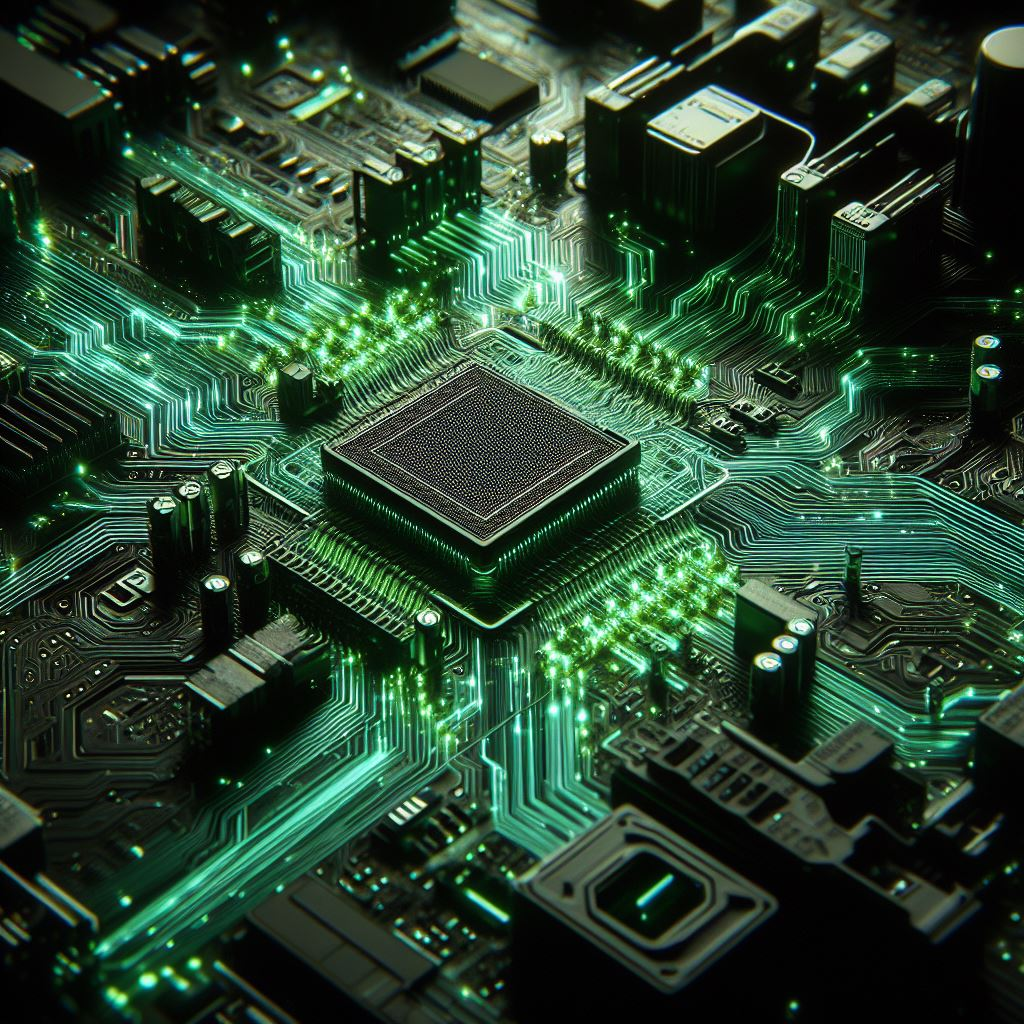
\includegraphics[width=0.4\linewidth]{Imagenes/buses.jpeg}
	\caption{Los circuitos integrados dar un salto en potencia y complejidad a los computadores.}
	\label{fig:enter-label}
\end{figure}

Durante esta generación, los sistemas operativos evolucionaron significativamente. Surgieron conceptos como la multiprogramación, que permitía que múltiples programas se ejecutaran al mismo tiempo, mejorando la utilización de la CPU. También se desarrollaron los sistemas de tiempo compartido, que permitían a múltiples usuarios interactuar con la computadora simultáneamente, lo que optimizó el uso de los recursos y facilitó el acceso a la computación.

Los lenguajes de programación de alto nivel continuaron evolucionando, y COBOL (Common Business-Oriented Language) se popularizó en el ámbito empresarial. Este lenguaje facilitó la programación de aplicaciones de gestión y negocios, ampliando el alcance de las computadoras en el sector comercial.

\subsection{La cuarta generación (1980 a la fecha): las computadoras personales}


La cuarta generación de computadoras comenzó en la década de 1980 con la aparición de los microprocesadores, que integraron la CPU completa en un solo chip. Esto permitió la creación de computadoras personales (PC) asequibles y potentes, accesibles para el uso doméstico y empresarial.
\begin{figure}[H]
	\centering
	
\includegraphics[width=0.4\linewidth]{Imagenes/computer.png}
	\caption{Desde los 80 en adelante, se popularizan las computadoras personales.}
	\label{fig:enter-label}
\end{figure}

Durante esta generación, los sistemas operativos avanzaron enormemente. Surgieron sistemas operativos gráficos como Windows y macOS, que hicieron que las computadoras fueran más fáciles de usar y accesibles para el público en general. La multitarea se convirtió en una característica estándar, permitiendo a los usuarios ejecutar múltiples aplicaciones simultáneamente.

La conectividad a internet se volvió omnipresente, transformando la forma en que las computadoras se utilizan para la comunicación, el comercio y el entretenimiento. Surgieron nuevas tecnologías como la computación en la nube, que permitieron el acceso remoto a recursos y servicios, y la inteligencia artificial, que comenzó a integrarse en diversas aplicaciones.

La popularización de los dispositivos móviles, como los smartphones y las tabletas, también marcó esta era, extendiendo las capacidades de las computadoras personales a dispositivos más portátiles y versátiles.




\section{Técnicas de mejora de rendimiento utilizadas en los sistemas operativos}
A medida que los sistemas operativos evolucionaban, se desarrollaron técnicas avanzadas para optimizar el uso de los recursos de hardware. Estas técnicas permitieron un mejor rendimiento y eficiencia en la gestión de tareas y recursos. Entre ellas se encuentran:

\subsection{Offline Processing}

\textbf{Descripción:} Permite procesar trabajos en lotes sin intervención del usuario. Los trabajos se preparan y almacenan para ser ejecutados posteriormente, optimizando el uso del tiempo de la CPU y otros recursos del sistema.

\textbf{Ejemplo:} Actualizaciones de Windows programadas para ejecutarse durante la noche.

\subsection{Buffering}
\textbf{Descripción:} Utiliza una memoria intermedia (buffer) para almacenar temporalmente datos durante las operaciones de entrada/salida (E/S). Esto permite que la CPU y los dispositivos de E/S trabajen de manera más eficiente y simultánea.

\textbf{Funcionamiento:} Mientras el dispositivo de E/S procesa un bloque de datos, la CPU puede seguir trabajando con otros datos almacenados en el buffer.

\textbf{Ejemplo: }Al ver un video en streaming, los datos se almacenan en un buffer antes de ser reproducidos, asegurando una reproducción continua sin interrupciones.

\subsection{Spooling (Simultaneous Peripheral Operations On-Line)}

\textbf{Descripción:} Almacena trabajos de E/S en una cola en el disco para ser procesados secuencialmente. Es especialmente útil para dispositivos que no pueden manejar múltiples tareas simultáneamente, como las impresoras.

\textbf{Funcionamiento:} Los documentos enviados a imprimir se almacenan en una cola en el disco (spool) y la impresora los procesa uno a uno en el orden en que llegaron.

\textbf{Ventajas:} Mejora la utilización de dispositivos periféricos, reduce el tiempo de espera y permite una gestión ordenada de los trabajos.

\textbf{Ejemplo:} En una oficina, varios usuarios envían trabajos de impresión simultáneamente. La técnica de spooling permite que estos trabajos se gestionen de manera eficiente y sin conflicto.

\section{Multiprogramación}
La multiprogramación es una técnica en la cual un sistema operativo permite que múltiples programas se ejecuten simultáneamente en una computadora. Esto se logra compartiendo el tiempo de la CPU entre varios programas, de modo que mientras un programa está esperando una operación de entrada/salida (como leer datos del disco), otro programa puede usar la CPU.

\subsection{Características de la Multiprogramación:}
\subsubsection{Maximización del Uso de la CPU}La CPU nunca está inactiva, siempre tiene trabajo que hacer.
\subsubsection{Gestión de Recursos:} La memoria, el almacenamiento y los dispositivos de E/S se gestionan de manera eficiente para que varios programas puedan ejecutarse sin interferencias.
\subsubsection{Context Switching:} El sistema operativo cambia rápidamente entre programas, lo que permite que varios programas parezcan ejecutarse al mismo tiempo.

\textbf{Ejemplos}

\textbf{Sistema Bancario:} Un banco puede procesar múltiples transacciones simultáneamente. Mientras una transacción espera la confirmación de una operación, otra transacción puede ser procesada.

\textbf{Uso Personal:} En una computadora personal, puedes escuchar música, descargar un archivo y escribir un documento al mismo tiempo gracias a la multiprogramación.

La multiprogramación es una base fundamental de los sistemas operativos modernos, permitiendo una utilización más eficiente y efectiva de los recursos de la computadora.

\section{Tiempo compartido (Time sharing)}
El tiempo compartido es una técnica de gestión de recursos en sistemas operativos que permite que múltiples usuarios utilicen una computadora simultáneamente. Esto se logra dividiendo el tiempo de la CPU en pequeños segmentos y asignando cada segmento a diferentes tareas o usuarios. Aquí están los puntos clave:
\begin{itemize}
	\item \textbf{Multiplicidad de usuarios:}  Varios usuarios pueden interactuar con el sistema al mismo tiempo.
	\item \textbf{Interactividad:}  Proporciona respuestas rápidas a cada usuario, creando la ilusión de acceso exclusivo.
	\item  \textbf{Gestión de recursos:} El sistema operativo gestiona la asignación de CPU, memoria y dispositivos de E/S entre las tareas.
\end{itemize}
\subsection{Funcionamiento}
\begin{itemize}
	\item \textbf{Slices de Tiempo}: La CPU se divide en pequeños intervalos de tiempo llamados "slices" o "quantums".
	\item \textbf{Asignación}: Cada usuario o tarea recibe un slice de tiempo, y la CPU alterna rápidamente entre ellos.
	\item \textbf{Interrupciones}: Al finalizar el slice de tiempo, una interrupción cambia el control de la CPU al siguiente usuario o tarea en cola.
\end{itemize}

\section{Tiempo real (Real time)}
El tiempo real en sistemas operativos se refiere a la capacidad de procesar datos y eventos de forma inmediata o dentro de un plazo específico y predecible. Los sistemas de tiempo real están diseñados para aplicaciones donde es crucial que las respuestas se entreguen sin demoras significativas. Aquí están los puntos clave:

\begin{itemize}
	\item \textbf{Determinismo}: Garantiza que las tareas se completen dentro de un tiempo específico.
	\item \textbf{Prioridades}: Asigna prioridades a las tareas, asegurando que las de mayor importancia se procesen primero.
	\item \textbf{Ejemplos}: Control de sistemas industriales, aviación, telecomunicaciones, y dispositivos médicos.
\end{itemize}
\section{Proceso distribuido}
Un proceso distribuido se refiere a un sistema en el que múltiples computadoras trabajan juntas para completar tareas o resolver problemas. Este enfoque distribuye la carga de trabajo entre varias máquinas, mejorando la eficiencia y la capacidad de procesamiento.

\subsection{Características}
\begin{itemize}
	\item \textbf{Descentralización}: No hay un único punto de control, lo que aumenta la robustez y la fiabilidad del sistema.
	\item \textbf{Concurrencia}: Múltiples procesos pueden ejecutarse simultáneamente en diferentes máquinas.
	\item \textbf{Escalabilidad}: Es fácil agregar más computadoras para aumentar la capacidad de procesamiento.
	\item \textbf{Fallo Tolerante}: Si una máquina falla, las otras pueden continuar con el trabajo, mejorando la resiliencia.
\end{itemize}

\subsection{Ejemplos}
\begin{itemize}
	\item \textbf{Sistemas de Archivos Distribuidos}: Almacenan datos en varias computadoras, permitiendo acceso rápido y redundante.
	\item \textbf{Computación en la Nube}: Proveedores como AWS, Google Cloud y Azure utilizan procesos distribuidos para ofrecer servicios de alta disponibilidad y escalabilidad.
	\item \textbf{Aplicaciones Web}: Sitios web de alto tráfico utilizan múltiples servidores para manejar solicitudes simultáneas y mejorar el rendimiento.
\end{itemize}

\section{Multiproceso}
El multiproceso es una técnica utilizada en sistemas operativos que permite ejecutar múltiples procesos simultáneamente utilizando más de una unidad central de procesamiento (CPU) o núcleo de CPU. Esto mejora significativamente el rendimiento y la eficiencia del sistema.

\subsection{Características}
\begin{itemize}
	\item \textbf{Paralelismo}: Los procesos se ejecutan en paralelo, utilizando múltiples CPUs o núcleos.
	\item \textbf{Independencia}: Cada proceso puede ejecutarse de manera independiente, sin afectar a los demás.
	\item \textbf{Escalabilidad}: Añadir más CPUs o núcleos mejora el rendimiento del sistema.
\end{itemize}

\subsection{Ventajas}
\begin{itemize}
	\item \textbf{Mejora del Rendimiento}: Permite realizar múltiples tareas al mismo tiempo, aumentando la velocidad de procesamiento.
	\item \textbf{Mayor Eficiencia}: Utiliza mejor los recursos del sistema, distribuyendo la carga de trabajo entre varias CPUs.
\end{itemize}

\subsection{Ejemplos}
\begin{itemize}
	\item \textbf{Servidores Web}: Manejan múltiples solicitudes de usuarios simultáneamente.
	\item \textbf{Aplicaciones Científicas}: Realizan cálculos complejos en paralelo, acelerando el tiempo de procesamiento.
	\item \textbf{Juegos y Software de Diseño}: Utilizan múltiples núcleos para gráficos y cálculos intensivos.
\end{itemize}

\subsection*{Comparación con la Multiprogramación}
\begin{itemize}
	\item \textbf{Multiprogramación}: Utiliza una sola CPU para ejecutar múltiples tareas, alternando rápidamente entre ellas.
	\item \textbf{Multiproceso}: Utiliza múltiples CPUs o núcleos para ejecutar tareas en paralelo, lo que permite un verdadero procesamiento simultáneo.
\end{itemize}


	%\chapter{Unidad 2. Estructuras del sistema operativo}

\section{Introducción}
El diseño de un sistema operativo depende en gran medida de su finalidad y del tipo de procesos que se desean realizar. Además, es crucial tener en cuenta las necesidades o requisitos del usuario y del propio software.
 A continuación, se detallan estos aspectos fundamentales:

\subsection{Finalidad del Sistema Operativo}

La finalidad de un sistema operativo puede variar según el contexto y los objetivos específicos para los cuales se diseñe. Algunas finalidades comunes incluyen:

\begin{itemize}
	\item \textbf{Gestión de Recursos}: Coordinar y optimizar el uso de los recursos de hardware (CPU, memoria, dispositivos de E/S) para mejorar el rendimiento y la eficiencia del sistema.
	\item \textbf{Interfaz de Usuario}: Proveer una interfaz amigable para que los usuarios interactúen fácilmente con el hardware y el software de la computadora.
	\item \textbf{Seguridad y Protección}: Asegurar que los datos y recursos del sistema estén protegidos contra accesos no autorizados y errores.
	\item \textbf{Compatibilidad y Soporte de Aplicaciones}: Facilitar la ejecución de aplicaciones y programas, proporcionando una plataforma estable y compatible.
\end{itemize}

\subsection{ Tipo de Procesos}

El tipo de procesos que se desea realizar influye significativamente en el diseño del sistema operativo. Algunos ejemplos incluyen:

\begin{itemize}
	\item \textbf{Procesamiento por Lotes}: Adecuado para tareas que pueden agruparse y ejecutarse sin intervención del usuario. Ejemplos: procesamiento de datos en bancos y grandes corporaciones.
	\item \textbf{Tiempo Compartido}: Permite que múltiples usuarios utilicen el sistema simultáneamente, cada uno con la ilusión de tener acceso exclusivo. Ejemplos: sistemas multiusuario en universidades y centros de investigación.
	\item \textbf{Tiempo Real}: Requiere que las operaciones se realicen dentro de un tiempo específico y predecible. Ejemplos: sistemas de control industrial, aviación, y dispositivos médicos.
	\item \textbf{Procesamiento Distribuido}: Involucra la coordinación de múltiples sistemas para trabajar en conjunto. Ejemplos: computación en la nube, sistemas de archivos distribuidos.
\end{itemize}

\subsection{Necesidades del Usuario}

Las necesidades del usuario pueden variar dependiendo del contexto de uso del sistema operativo. Algunas necesidades comunes incluyen:

\begin{itemize}
	\item \textbf{Facilidad de Uso}: Interfaces gráficas intuitivas y fáciles de navegar.
	\item \textbf{Personalización}: Opciones para personalizar el entorno de trabajo según las preferencias del usuario.
	\item \textbf{Soporte Técnico y Documentación}: Acceso a soporte técnico y documentación detallada para resolver problemas y aprender a usar el sistema.
	\item \textbf{Compatibilidad de Software}: Capacidad para ejecutar una amplia variedad de aplicaciones y software específico del usuario.
\end{itemize}

\subsection{ Necesidades del Software}

El software que se ejecutará en el sistema operativo también impone requisitos específicos que deben ser considerados en el diseño. Algunos de estos requisitos incluyen:

\begin{itemize}
	\item \textbf{Gestión de Memoria}: Necesidad de un manejo eficiente de la memoria para ejecutar aplicaciones grandes y complejas.
	\item \textbf{Procesamiento Multitarea}: Capacidad para ejecutar múltiples tareas simultáneamente sin degradación del rendimiento.
	\item \textbf{Control de Dispositivos}: Soporte para una variedad de dispositivos de entrada/salida, como impresoras, escáneres, y dispositivos de almacenamiento externo.
	\item \textbf{Seguridad y Protección de Datos}: Implementación de medidas de seguridad para proteger los datos y asegurar la integridad del sistema.
\end{itemize}



\subsection*{Modos Usuario y Kernel del Sistema Operativo}

\textbf{Modo Usuario}

\begin{itemize}
	\item \textbf{Descripción}: 
	\begin{itemize}
		\item El modo usuario es el modo de operación en el que se ejecutan las aplicaciones y programas del usuario.
		\item Las aplicaciones en este modo tienen acceso limitado a los recursos del sistema y no pueden realizar operaciones críticas de hardware directamente.
		\item El sistema operativo proporciona una capa de protección para evitar que las aplicaciones en modo usuario dañen el sistema o interfieran con otras aplicaciones.
	\end{itemize}

\end{itemize}

\textbf{Modo Kernel}

\begin{itemize}
	\item \textbf{Descripción}:
	\begin{itemize}
		\item El modo kernel es el modo de operación en el que se ejecuta el núcleo del sistema operativo.
		\item Tiene acceso completo a todos los recursos del hardware, incluyendo la memoria, el procesador y los dispositivos de entrada/salida.
		\item Las operaciones críticas del sistema, como la gestión de procesos, la gestión de memoria y el control de dispositivos, se realizan en este modo.
	\end{itemize}

\end{itemize}

\textbf{Comparación}

\begin{itemize}
	\item \textbf{Seguridad}:
	\begin{itemize}
		\item \textbf{Modo Usuario}: Mayor seguridad debido a las restricciones de acceso.
		\item \textbf{Modo Kernel}: Menor seguridad ya que tiene acceso total a los recursos.
	\end{itemize}
	\item \textbf{Acceso a Recursos}:
	\begin{itemize}
		\item \textbf{Modo Usuario}: Acceso limitado; requiere llamadas al sistema para servicios.
		\item \textbf{Modo Kernel}: Acceso completo y directo a todos los recursos del sistema.
	\end{itemize}
	\item \textbf{Propósito}:
	\begin{itemize}
		\item \textbf{Modo Usuario}: Ejecutar aplicaciones y programas del usuario.
		\item \textbf{Modo Kernel}: Gestionar y controlar el hardware y los recursos del sistema.
	\end{itemize}
\end{itemize}


 

\section{Estructura monolítica}

Es la estructura de los primeros sistemas operativos, constituidos fundamentalmente por un solo programa compuesto de un conjunto de rutinas entrelazadas de tal forma que cada una puede llamar a cualquier otra.

\begin{figure}[H]
	\centering
	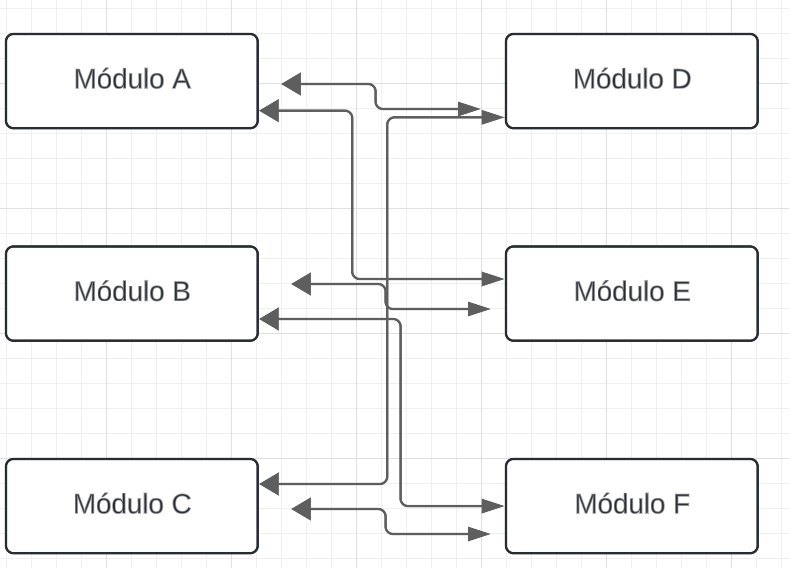
\includegraphics[width=0.6\linewidth]{Imagenes/monolitico.png}
	\caption{En un sistema operativo monolítico sus módulos están entrelazados. }
	\label{fig:enter-label}
\end{figure}

\subsection{Características Fundamentales del Sistema Monolítico}
\begin{tcolorbox}

\subsubsection{Estructura Unificada}
\begin{itemize}
	\item \textbf{Descripción}: El sistema operativo monolítico se compone de un único bloque de código en el que todos los servicios del sistema (gestión de archivos, gestión de memoria, manejo de dispositivos, etc.) están interrelacionados.
	\item \textbf{Funcionalidad}: Todas las funciones del sistema operativo están disponibles en el mismo espacio de direcciones y pueden llamarse entre sí directamente.
\end{itemize}
	
\end{tcolorbox}


\begin{tcolorbox}


\subsubsection{Rendimiento Alto}
\begin{itemize}
	\item \textbf{Descripción}: Al tener todos los servicios en un único espacio de direcciones, las llamadas de función son rápidas.
	\item \textbf{Ventaja}: No hay necesidad de cambiar entre el modo usuario y el modo kernel para acceder a los servicios del sistema operativo, lo que reduce la sobrecarga y mejora el rendimiento.
\end{itemize}
\end{tcolorbox}

\begin{tcolorbox}

\subsubsection{Simplicidad de Implementación}
\begin{itemize}
	\item \textbf{Descripción}: La estructura monolítica es más sencilla de implementar y gestionar, ya que todo el código está contenido en un solo lugar.
	\item \textbf{Beneficio}: Esto facilita la integración de componentes y la comunicación interna, haciendo que el desarrollo inicial del sistema operativo sea más directo.
\end{itemize}

\end{tcolorbox}


\begin{tcolorbox}
	
\subsubsection{Dificultad en la Escalabilidad}
\begin{itemize}
	\item \textbf{Descripción}: Agregar nuevas funciones o servicios puede ser complicado debido a la interdependencia entre los componentes existentes.
	\item \textbf{Reto}: A medida que el sistema operativo crece, mantener y extender el código puede volverse más complejo.
\end{itemize}

\end{tcolorbox}

\begin{tcolorbox}
\subsubsection{Seguridad Reducida}
\begin{itemize}
	\item \textbf{Descripción}: La falta de separación entre los distintos componentes del sistema operativo implica que un fallo en un módulo puede comprometer todo el sistema.
	\item \textbf{Consecuencia}: Esto reduce la robustez y la seguridad del sistema operativo, ya que cualquier error puede afectar a todo el sistema.
\end{itemize}
\end{tcolorbox}


\section{Estructura Jerárquica}



La estructura jerárquica llega como una evolución natural de los sistemas operativos. A medida que crecieron las necesidades de los usuarios y aumentó la complejidad de las aplicaciones, se hizo necesaria una mejor organización del software. 

La estructura jerárquica organiza el sistema operativo en pequeñas partes o capas, cada una de las cuales tiene una función específica y depende de las capas inferiores para realizar sus tareas.
Uno de los ejemplos más conocidos de estructura jerárquica es el modelo THE (Technische Hogeschool, Eindhoven  ) desarrollado por Edsger Dijkstra, y se presenta de la siguiente manera:
\begin{figure}[H]
	\centering
	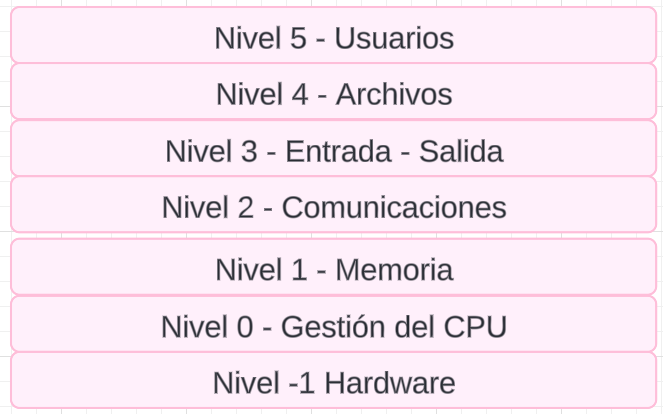
\includegraphics[width=0.6\linewidth]{Imagenes/jerarquico.png}
	\caption{En un sistema operativo monolítico sus módulos están entrelazados. }
	\label{fig:enter-label}
\end{figure}



En la estructura jerárquica, el sistema operativo se divide en capas, donde cada capa proporciona servicios a la capa superior y utiliza los servicios de la capa inferior. La capa más baja interactúa directamente con el hardware, y la capa más alta proporciona la interfaz de usuario.

\begin{tcolorbox}[title=Capas de la estructura jerárquica]


\begin{itemize}
	\item \textbf{Capa -1 (Hardware)}
	\begin{itemize}
		\item \textbf{Función}: Interactúa directamente con el hardware físico del sistema, incluyendo la CPU, la memoria y los dispositivos de E/S.
	\end{itemize}
	
	\item \textbf{Capa 0 (Planificación del Procesador)}
	\begin{itemize}
		\item \textbf{Función}: Controla la ejecución de procesos y la planificación de tareas. Gestiona la creación, terminación y sincronización de procesos.
	\end{itemize}
	
	\item \textbf{Capa 1 (Gestión de la Memoria)}
	\begin{itemize}
		\item \textbf{Función}: Maneja la asignación y el control de la memoria. Proporciona servicios como la asignación de memoria y el intercambio de memoria.
	\end{itemize}
	
	\item \textbf{Capa 2 (Controlador de la Consola de Operador)}
	\begin{itemize}
		\item \textbf{Función}: Gestiona la interacción con la consola del operador, permitiendo la entrada y salida de comandos y datos.
	\end{itemize}
	
	\item \textbf{Capa 3 (Control de Entrada/Salida)}
	\begin{itemize}
		\item \textbf{Función}: Controla los dispositivos de hardware a través de controladores. Gestiona las operaciones de entrada/salida y la comunicación con los periféricos.
	\end{itemize}
	
	\item \textbf{Capa 4 (Gestión de Archivos)}
	\begin{itemize}
		\item \textbf{Función}: Proporciona servicios de sistema de archivos, como la creación, eliminación y manipulación de archivos. Controla el acceso a los datos almacenados en disco.
	\end{itemize}
	
	\item \textbf{Capa 5 (Control de Programas de Usuarios)}
	\begin{itemize}
		\item \textbf{Función}: Gestiona la ejecución y control de los programas de los usuarios, proporcionando una interfaz para la interacción con el sistema operativo.
	\end{itemize}
\end{itemize}
\end{tcolorbox}
\subsection{Características Fundamentales}


\begin{itemize}
	\item \textbf{Modularidad}
	\begin{itemize}
		\item \textbf{Descripción}: Cada capa del sistema operativo está diseñada para cumplir con una función específica, permitiendo que los desarrolladores trabajen en una capa sin afectar las demás.
		\item \textbf{Ventaja}: Facilita el desarrollo, la prueba y el mantenimiento del sistema operativo.
	\end{itemize}
	
	\item \textbf{Independencia de Capas}
	\begin{itemize}
		\item \textbf{Descripción}: Las capas superiores dependen de los servicios proporcionados por las capas inferiores, pero no necesitan conocer los detalles internos de esas capas.
		\item \textbf{Ventaja}: Mejora la confiabilidad y la seguridad del sistema, ya que los cambios en una capa no afectan a las demás.
	\end{itemize}
	
	\item \textbf{Facilidad de Mantenimiento}
	\begin{itemize}
		\item \textbf{Descripción}: La modularidad y la independencia de capas hacen que el sistema operativo sea más fácil de mantener y actualizar.
		\item \textbf{Ventaja}: Las actualizaciones y correcciones de errores pueden realizarse en una capa sin afectar el resto del sistema.
	\end{itemize}
\end{itemize}

\section{Máquina Virtual}
La máquina virtual es una evolución natural de los sistemas operativos que aprovecha la potencia del hardware moderno para aplicar la técnica de multiprogramación y el concepto de máquina extendida. 

Una máquina extendida es una versión virtualizada de una computadora física que presenta una visión más completa y rica de los recursos de hardware. En lugar de interactuar directamente con el hardware físico, los programas y sistemas operativos interactúan con una representación virtual de la máquina.

\begin{figure}[H]
	\centering
	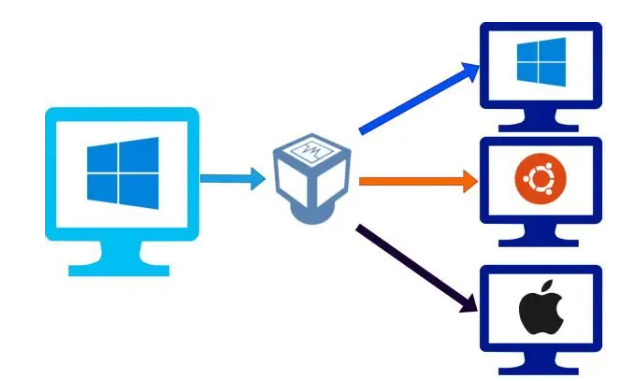
\includegraphics[width=0.6\linewidth]{Imagenes/virtual.png}
	\caption{Una máquina virtual puede ejecutar diferentes s.o. en una computadora. }
	\label{fig:enter-label}
\end{figure}


 Esto permite la integración de distintos sistemas operativos en una sola computadora física, dando la sensación de tener varias máquinas diferentes y permitiendo la ejecución simultánea de múltiples sistemas operativos y aplicaciones.
 
\subsection{Características Fundamentales
}


\begin{itemize}
	\item \textbf{Aislamiento}
	\begin{itemize}
		\item \textbf{Descripción}: Cada máquina virtual es como una burbuja separada, sin afectar a las otras burbujas.
		\item \textbf{Ventaja}: Si una máquina virtual falla, las otras siguen funcionando sin problemas.
	\end{itemize}
	
	\item \textbf{Flexibilidad}
	\begin{itemize}
		\item \textbf{Descripción}: Puedes ejecutar diferentes sistemas operativos al mismo tiempo en la misma computadora.
		\item \textbf{Ventaja}: Esto es útil para pruebas y desarrollo, ya que no necesitas hardware adicional.
	\end{itemize}
	
	\item \textbf{Eficiencia de Recursos}
	\begin{itemize}
		\item \textbf{Descripción}: El monitor de recursos distribuye los recursos (como CPU y memoria) de manera eficiente entre las máquinas virtuales.
		\item \textbf{Ventaja}: Se aprovecha mejor el hardware de la computadora.
	\end{itemize}
	
\end{itemize}

\section{Estructura Cliente-Servidor}



El modelo cliente-servidor es una arquitectura de sistemas operativos y aplicaciones donde las tareas se reparten entre proveedores de recursos o servicios, llamados servidores, y los consumidores de esos servicios, llamados clientes. Este modelo es ampliamente utilizado en redes y permite una distribución eficiente de tareas y recursos.
\begin{figure}[H]
	\centering
	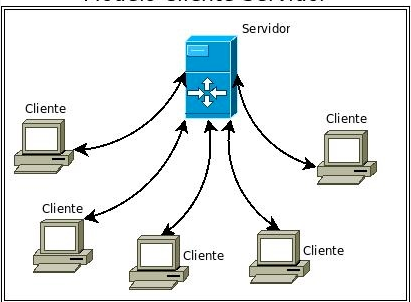
\includegraphics[width=0.7\linewidth]{Imagenes/cliente-servidor.png}
	\caption{El modelo cliente-servidor. }
	\label{fig:enter-label}
\end{figure}


En un sistema operativo cliente-servidor, los servidores son programas que proporcionan servicios específicos, como almacenamiento de datos, procesamiento de aplicaciones, o administración de recursos. Los clientes son programas que solicitan estos servicios. La comunicación entre clientes y servidores se realiza a través de una red.

\subsection{Características Fundamentales}

\begin{itemize}
	\item \textbf{Distribución de Tareas}
	\begin{itemize}
		\item \textbf{Descripción}: Las tareas se reparten entre clientes y servidores. Los servidores gestionan y proporcionan recursos y servicios, mientras que los clientes consumen estos servicios.
		\item \textbf{Ventaja}: Mejora la eficiencia y permite la especialización en la provisión de servicios.
	\end{itemize}
	
	\item \textbf{Independencia de Plataforma}
	\begin{itemize}
		\item \textbf{Descripción}: Los clientes y servidores pueden operar en diferentes plataformas de hardware y sistemas operativos, siempre que se adhieran a protocolos de comunicación comunes.
		\item \textbf{Ventaja}: Facilita la integración de diferentes tecnologías y sistemas.
	\end{itemize}
	
	\item \textbf{Escalabilidad}
	\begin{itemize}
		\item \textbf{Descripción}: Es fácil agregar más servidores o clientes según la demanda, permitiendo una escalabilidad horizontal.
		\item \textbf{Ventaja}: Permite manejar incrementos en la carga de trabajo de manera eficiente.
	\end{itemize}
	
	\item \textbf{Mantenimiento Centralizado}
	\begin{itemize}
		\item \textbf{Descripción}: La gestión y el mantenimiento de los recursos y servicios se centralizan en los servidores.
		\item \textbf{Ventaja}: Facilita la administración y el mantenimiento del sistema.
	\end{itemize}
\end{itemize}

\subsubsection*{Ejemplo de Funcionamiento}

En un sistema cliente-servidor, los clientes envían solicitudes a los servidores a través de la red. Los servidores procesan estas solicitudes y envían las respuestas correspondientes. Por ejemplo:
\begin{itemize}
	\item Un cliente puede solicitar datos de una base de datos al servidor.
	\item El servidor procesa la solicitud, accede a la base de datos, y envía los datos solicitados al cliente.
\end{itemize}

\section{Prestaciones de un sistema operativo}
Se ha mencionado que la misión del sistema operativo es ayudar al usuario con el manejo de la computadora, para eso debe proporcionar ciertos servicios que se pueden considerar desde dos puntos de vista distintos.

\begin{tcolorbox}
\begin{itemize}
	\item Punto de vista del programador
	\item Punto de vista del sistema
\end{itemize}

\end{tcolorbox}

\subsubsection{Punto de vista del programador}
Desde el punto de vista del programador, las prestaciones del sistema operativo son las funcionalidades y servicios que el sistema operativo proporciona para facilitar el desarrollo, ejecución y gestión de programas. 

Estas prestaciones permiten a los programadores enfocarse en la lógica y funcionalidad de sus aplicaciones sin tener que preocuparse por los detalles del hardware y la gestión de recursos subyacentes.

\begin{tcolorbox}
\textbf{Punto de vista del programador}:	funcionalidades del sistema operativo, que facilitan el desarrollo, la ejecución, y gestión de programas.

\subsubsection{Ejecución de programas}
\begin{itemize}
	\item El sistema operativo proporciona servicios que permiten cargar, ejecutar y finalizar programas de manera eficiente.
\end{itemize}

\subsubsection{Operaciones de Entrada/Salida (E/S)}
\begin{itemize}
	\item El sistema operativo maneja las operaciones de entrada y salida, facilitando la interacción entre el software y los dispositivos de hardware.
\end{itemize}

\subsubsection{Gestión de archivos}
\begin{itemize}
	\item El sistema operativo proporciona mecanismos para la creación, acceso y manipulación de archivos en el sistema de archivos.
\end{itemize}

\end{tcolorbox}


\subsubsection{Punto de vista del sistema}
Desde el punto de vista del sistema, las prestaciones del sistema operativo se centran en cómo se gestionan y optimizan los recursos del sistema para garantizar su eficiencia, seguridad y estabilidad. 
\begin{tcolorbox}
	\textbf{Punto de vista del sistema}: Gestión y optimización de recursos.
	
	\subsubsection{Asignación de Recursos}
	\begin{itemize}
		\item La asignación de recursos implica distribuir de manera eficiente la CPU, memoria y otros recursos del sistema entre los programas que se están ejecutando, resolviendo conflictos de asignación cuando varios procesos o usuarios compiten por los mismos recursos.
	\end{itemize}
	
	\subsubsection{Contabilidad}
	\begin{itemize}
		\item La contabilidad en un sistema operativo se refiere al registro y monitoreo del uso de recursos por parte de los diferentes procesos y usuarios.
	\end{itemize}
	
	\subsubsection{Protección}
	\begin{itemize}
		\item La protección en un sistema operativo implica asegurar que los datos y recursos del sistema no sean accesibles de manera indebida o por usuarios no autorizados.
	\end{itemize}
	
\end{tcolorbox}

\subsection{Servicios de usuario}
El sistema operativo ofrece servicios a los usuarios de dos formas diferentes: a través de llamadas al sistema operativo desde un proceso y mediante la ejecución de programas del propio sistema operativo. 

	\subsubsection{Llamadas al sistema operativo desde un proceso}
Las llamadas al sistema operativo son interfaces que permiten a los programas solicitar servicios específicos del sistema operativo. Estas llamadas se agrupan en varias categorías:
\begin{tcolorbox} 
	
		\begin{enumerate}
			\item\textbf{ Gestión de procesos}: Permiten crear, gestionar y terminar procesos. 
			\begin{lstlisting}
				exit()
			\end{lstlisting}
			
			\textit{Cuando cierras una aplicación.}
			 \item \textbf{Gestión de operaciones de E/S}: Permiten realizar operaciones de entrada y salida.
		\begin{lstlisting}
			read()
		\end{lstlisting}
		\textit{Cuando abres un archivo de word.}

		
		\item \textbf{Gestión de sistema de archivos}: Permiten manipular archivos y directorios. 
		\begin{lstlisting}
			mkdir ejemplo
		\end{lstlisting}
		
		\textit{Cuando creas una carpeta.}
		\end{enumerate}

\end{tcolorbox}
	
	
	\subsubsection{Ejecución de programas del propio sistema operativo}
	Además de las funciones básicas del núcleo que pueden ser ejecutadas por medio de llamadas al sistema, el sistema operativo proporciona un conjunto de programas cuya misión es resolver problemas comunes de los usuarios. 
	
	Estos programas se agrupan en varias categorías y facilitan la interacción con el sistema, proporcionando herramientas útiles para la gestión y manipulación de datos.
	
	\begin{tcolorbox}
	\begin{enumerate}
	\item\textbf{Tratamiento de Archivos }:Programas que permiten manipular archivos, tales como copiar, mover, renombrar y eliminar archivos.

	\begin{lstlisting}
		cp ejemplo.txt ejemplo1.txt
	\end{lstlisting}
	 \textit{Copia archivos de un lugar a otro}
	 
	 \item \textbf{Información}: Programas que proporcionan información sobre el sistema y los archivos, ayudando a los usuarios a entender el estado y uso de los recursos del sistema. 

		\begin{lstlisting}
		ls %Lista los archivos en un directorio
		df %Muestra el espacio disponible en disco
	\end{lstlisting}
	

	
	\item \textbf{Editores}:  Programas que permiten editar archivos de texto, proporcionando interfaces desde simples a muy sofisticadas. 

	\begin{lstlisting}
		nano ejemplo.txt
	\end{lstlisting}
	\textit{Cuando creas una carpeta.}
	
	\item \textbf{Ejecución}: Programas que permiten ejecutar y gestionar otros programas.
		\begin{lstlisting}
		python ejemplo.py
		sh script.sh
	\end{lstlisting}
	
		\item \textbf{Interprete de comandos}: Programas que interpretan y ejecutan comandos ingresados por el usuario, proporcionando una interfaz interactiva para el control del sistema.
	\begin{lstlisting}
		$ bash
		$ echo "Hola, mundo!"
		$ ls -la
	\end{lstlisting}
	
		\item \textbf{Programas de utilidad}: Programas que realizan tareas comunes de mantenimiento y gestión del sistema.
	\begin{lstlisting}
		$ grep "hola" ejemplo.txt
		$ Busca la palabra "hola" en el archivo
		
	\end{lstlisting}
\end{enumerate}
	

\end{tcolorbox}

\subsection{Servicios del sistema}

El sistema operativo actúa como un programa activado por eventos, respondiendo a diversas llamadas del sistema y manejando interrupciones y excepciones.
\subsubsection{Llamadas al sistema operativo}
	
Las llamadas al sistema operativo se agrupan según el tipo de llamada y  no por las acciones que realizan. Estas llamadas permiten a los programas interactuar con el núcleo del sistema operativo para realizar operaciones específicas.

	\begin{tcolorbox}
	\begin{enumerate}
		\item\textbf{Terminación normal }:Llamadas que permiten a un proceso finalizar su ejecución de manera controlada.
		
		\begin{lstlisting}
			exit()
		\end{lstlisting}
		\textit{El comando exit() es una llamada que finaliza el proceso actual y libera los recursos asignados.}
		
		\item\textbf{Terminación anormal }: Ocurre cuando un proceso termina debido a un error o una condición inesperada.
		
		\begin{lstlisting}
			Exception in thread "main" java.lang.NullPointerException
			at tu.paquete.TuClase.tuMetodo(TuClase.java:numeroDeLinea)
		\end{lstlisting}
		
		
		
		\textit{Cuando un programa Java intenta utilizar un objeto que no ha sido inicializado (es decir, que apunta a null), se lanza una NullPointerException. }
		
		\item \textbf{Peticiones de estado}: Llamadas que solicitan información sobre el estado del sistema, procesos u otros recursos. Se procesa la petición solicitada y se devuelve el control al programa que la solicitó.
		
		\begin{lstlisting}
			# Obtener el ID del proceso actual
			pid=$$
			# Imprimir el ID del proceso actual
			echo "El ID del proceso actual es: $pid"
		\end{lstlisting}
		
		
		
		\item \textbf{Peticiones de recursos}:  Los programas que son ejecutados, solicitan la asignación o liberación de recursos, y serán atendidos inmediatamente o entrarán en un estado de espera hasta ser atendidos.
	
		
		\item \textbf{Peticiones de E/S}: Llamadas que solicitan operaciones de entrada/salida, como leer o escribir datos.
		\begin{lstlisting}
			nombre = input('ingrese su nombre')
			print(nombre)
		\end{lstlisting}
		
	
	\end{enumerate}
	
	
\end{tcolorbox}

\subsubsection{Interrupciones de los Dispositivos de E/S}
Las interrupciones son señales enviadas por dispositivos de E/S al procesador para indicar que requieren atención. El sistema operativo maneja estas interrupciones y decide la acción a tomar.

Pueden ser:
	\begin{tcolorbox}
	\begin{enumerate}
		\item\textbf{Quedando en espera }:El proceso se suspende y espera a que el dispositivo esté listo para continuar. En este caso, el dispositivo externo, cuando termine la operación, producirá una interrupción que dará control al sistema operativo, el cual activará el proceso que estaba en espera.
		
	
		\textit{ \textbf{Ejemplo:} Un proceso que espera a que un disco duro termine de escribir datos antes de continuar con su ejecución.}
		
		\item\textbf{Siguiendo con las operaciones }:  El proceso principal continúa ejecutándose mientras el sistema operativo maneja las interrupciones en segundo plano. Esto permite que la computadora realice múltiples tareas al mismo tiempo.
		
	
		\textit{\textbf{Ejemplo}: Estás imprimiendo un documento mientras sigues trabajando en otros programas. La impresora envía una interrupción cuando termina de imprimir cada página, pero tu trabajo no se detiene. }
		
	
		
		
	\end{enumerate}
	
	
\end{tcolorbox}

\subsubsection{Gestión de excepciones}
La gestión de excepciones es un mecanismo para manejar condiciones excepcionales, como errores de hardware o software, que ocurren durante la ejecución de un programa.

\textit{El sistema operativo detecta la excepción, interrumpe la ejecución del programa, y ejecuta un manejador de excepciones.
}

\subsection{Protecciones del sistema operativo}
Las protecciones en el sistema operativo son funciones implementadas para evitar problemas entre procesos y entre estos y el propio sistema operativo. Estas protecciones aseguran que los procesos no interfieran entre sí y que el sistema operativo mantenga su integridad y estabilidad. Existen varios tipos de protecciones, entre las cuales se incluyen la protección de entrada/salida (E/S), la protección de memoria y la protección del procesador.


	\begin{enumerate}
			\begin{tcolorbox}
		\item\textbf{Protección de Entrada/Salida (E/S)}: Garantiza que las operaciones de E/S sean seguras y controladas, evitando que los procesos interfieran con los dispositivos de E/S de otros procesos. Solo los procesos autorizados pueden acceder a dispositivos de E/S específicos.
		
		\textit{ \textbf{Ejemplo:}Un sistema operativo que utiliza permisos para controlar el acceso a una impresora, asegurando que solo ciertos usuarios o procesos puedan enviar trabajos de impresión.}
		
		\item\textbf{Protección de Memoria}: Previene que los procesos accedan a áreas de memoria que no les pertenecen, evitando corrupción de datos y fallos del sistema.
		
			
		\item\textbf{Protección del Procesador}: Asegura que ningún proceso pueda monopolizar el procesador, garantizando una distribución justa del tiempo de CPU entre todos los procesos.
		Utiliza temporizadores y modos de operación (modo usuario y modo kernel) para controlar el uso del procesador.
		
		
	\end{tcolorbox}
		
	\end{enumerate}
	
	

 
















	%\chapter{Unidad 3. El núcleo y los procesos.}
El núcleo, conocido también como kernel, es el corazón del sistema operativo. Su función principal es gestionar de manera eficiente los recursos del sistema, como el procesador, la memoria, los dispositivos de entrada/salida (E/S), y otros recursos esenciales. El kernel actúa como intermediario entre el hardware y las aplicaciones que se ejecutan en el sistema, asegurando que los recursos se utilicen de manera óptima y que las aplicaciones puedan acceder a ellos de manera segura y controlada.

\begin{tcolorbox}
	\section{
		Funciones del Kernel}
	
	El kernel realiza varias funciones críticas en un sistema operativo:
	
	\textbf{Gestión del Procesador: }Coordina la asignación del tiempo de CPU a los diferentes procesos que se ejecutan en el sistema. Esto incluye la planificación de procesos y la conmutación de contexto entre procesos.
	
	\textbf{Gestión de la Memoria:} Supervisa y controla el acceso a la memoria principal. Esto incluye la asignación de memoria a los procesos, el manejo de la memoria virtual y la protección de la memoria para evitar que un proceso interfiera con otro.
	
	\textbf{
		Gestión de Entrada/Salida (E/S):} Controla las operaciones de entrada y salida, gestionando el acceso a dispositivos como discos duros, impresoras y otros periféricos. El kernel facilita la comunicación entre los dispositivos y los procesos que necesitan interactuar con ellos.
	
	\textbf{Gestión de Recursos: }Además de CPU, memoria y dispositivos de E/S, el kernel también administra otros recursos del sistema, como el sistema de archivos, la seguridad y la gestión de usuarios.


\end{tcolorbox}
\section{Procesos}

Uno de los conceptos más fundamentales en la gestión de un sistema operativo es el de \textbf{proceso}. El concepto de proceso se originó con la llegada de la \textit{multiprogramación}, que permitió la ejecución simultánea de múltiples programas en un mismo sistema. Esta capacidad transformó la forma en que los sistemas operativos gestionan los recursos y las tareas que se llevan a cabo en un ordenador.

Consideremos el caso de una computadora portátil moderna. Desde el momento en que se enciende, el sistema operativo comienza a ejecutar una serie de procesos en segundo plano, muchos de los cuales el usuario ni siquiera nota. Por ejemplo, se inician procesos como el explorador de Windows, servicios esenciales como los de red e impresión, procesos de seguridad como el antimalware, servidores de bases de datos, y la Máquina Virtual de Java (JVM) si el entorno está configurado para desarrollo con Java. Mientras estos procesos se ejecutan, el usuario puede estar navegando por internet o escuchando música, sin darse cuenta de la complejidad de las operaciones que ocurren simultáneamente.
\begin{figure}[H]
	\centering
	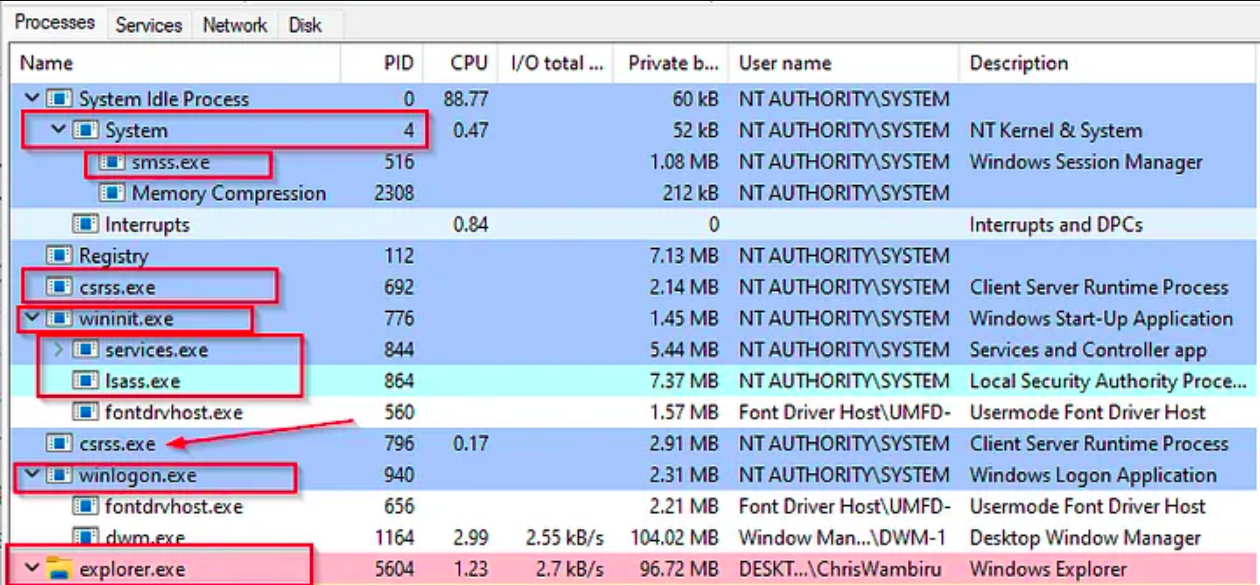
\includegraphics[width=0.8\linewidth]{Imagenes/procesos.png}
	\caption{Procesos que se inician al arrancar windows. }
	\label{fig:enter-label}
\end{figure}

Toda esta actividad debe ser gestionada de manera eficiente, y es aquí donde entra en juego la multiprogramación con soporte para múltiples procesos. Esta técnica permite que el sistema operativo administre los recursos del procesador, la memoria y otros dispositivos, de manera que varios procesos puedan ejecutarse ``al mismo tiempo'' sin interferir unos con otros.

Podemos, entonces, definir a un \textbf{proceso} como:

\begin{tcolorbox}
	\textbf{Una instancia de un programa en ejecución.}
\end{tcolorbox}

Un proceso no es solo un programa almacenado en disco o en la memoria, sino una entidad activa que está utilizando los recursos del sistema para llevar a cabo tareas específicas. Cada proceso tiene su propio espacio de memoria, su estado, y es gestionado por el sistema operativo para asegurar que todos los procesos puedan operar de manera eficiente y segura dentro del sistema.
\begin{table}[H]
	\centering
	\rowcolors{2}{gray!25}{white}
	\begin{tabularx}{0.9\textwidth}{|X|X|}
		\hline
		\textbf{Programa} & \textbf{Proceso} \\ \hline
		Conjunto de instrucciones almacenadas en disco o memoria. & Instancia de un programa en ejecución. \\ \hline
		Es un archivo pasivo, sin interacción con el hardware hasta que se ejecuta. & Es una entidad activa que utiliza recursos del sistema como CPU, memoria, etc. \\ \hline
		No tiene estado hasta que se inicia su ejecución. & Tiene un estado (listo, en ejecución, en espera, etc.) que cambia dinámicamente. \\ \hline
		Es estático, no cambia una vez escrito. & Es dinámico, ya que las instrucciones se están ejecutando y puede cambiar con el tiempo. \\ \hline
		Puede existir en disco duro o en memoria como código fuente o compilado. & Existe en la memoria principal y se asocia a un identificador único (PID). \\ \hline
		No consume recursos del sistema operativo por sí mismo. & Consume recursos como tiempo de CPU, espacio en memoria, y otros mientras se ejecuta. \\ \hline
	\end{tabularx}
	\caption{Diferencias entre un programa y un proceso}
	\label{tabla_programa_proceso}
\end{table}
\subsection{El modelo del proceso}

El modelo del proceso describe cómo el sistema operativo maneja la ejecución de programas. Este modelo es fundamental para entender cómo los programas se convierten en procesos activos en el sistema y cómo se gestionan durante su ciclo de vida.

En el modelo de procesos, cada proceso se concibe como una entidad que contiene:

\begin{itemize}
	\item \textbf{Código del programa}: Las instrucciones que el proceso ejecutará.
	\item \textbf{Datos}: Las variables necesarias para la ejecución.
	\item \textbf{Recursos del sistema}: CPU, memoria, dispositivos de E/S, que el proceso necesita para funcionar.
\end{itemize}

Para entender mejor el \textbf{modelo del proceso}, podemos utilizar la siguiente analogía de un taller mecánico:

\subsubsection{Analogía: Taller Mecánico}
\begin{tcolorbox}
	\begin{enumerate}
		\item \textbf{Vehículo en el Taller (Proceso):} Imagina que cada proceso es un vehículo que llega a un taller mecánico para ser reparado o mantenido. Este vehículo representa una instancia de un programa que ha sido \textit{activado} y ahora requiere atención.
		
		\item \textbf{Mecánico (Procesador):} El mecánico del taller es como el procesador del sistema, encargado de realizar las reparaciones necesarias. Este mecánico debe seguir un conjunto de instrucciones específicas (el programa) para reparar el vehículo.
		
		\item \textbf{Manual de Reparaciones (Programa):} El mecánico consulta un manual de reparaciones, que contiene todas las instrucciones necesarias para realizar la reparación. Este manual es análogo al código del programa que el proceso necesita ejecutar.
		
		\item \textbf{Herramientas y Piezas (Recursos del Sistema):} Para llevar a cabo las reparaciones, el mecánico necesita herramientas y piezas de recambio, que en el sistema operativo corresponden a los recursos del sistema, como la CPU, memoria, y dispositivos de entrada/salida.
		
		\item \textbf{Ejecución del Proceso:} Mientras el vehículo está en el taller, el mecánico trabaja en él, siguiendo el manual, utilizando las herramientas y asegurándose de que la reparación se realice correctamente. Esto es similar a cómo un proceso se ejecuta en un sistema operativo, siguiendo las instrucciones del programa y utilizando los recursos disponibles.
	\end{enumerate}
\end{tcolorbox}

La idea clave es que un proceso es una actividad de cierto tipo: tiene un programa, una entrada, una salida y un estado. Varios procesos pueden compartir un solo procesador mediante el uso de un algoritmo de planificación para determinar cuándo se debe detener el trabajo en un proceso para dar servicio a otro.


\subsection{Bloque de control de procesos (PCB)}

Desde el punto de vista del sistema operativo, un proceso se representa como un conjunto de datos que describe su estado en cada momento, los recursos utilizados, los registros, y otra información relevante. Este conjunto de datos se denomina \textbf{Bloque de control de procesos} (\textbf{PCB}, por sus siglas en inglés: \textit{Process Control Block}).

El PCB es fundamental para la gestión de procesos en un sistema operativo, ya que contiene toda la información necesaria para controlar y administrar un proceso. Cada proceso en el sistema tiene su propio PCB, y estos se almacenan en una estructura de datos que el sistema operativo utiliza para llevar un seguimiento preciso de todos los procesos.

A continuación, se detallan los componentes clave que suelen incluirse en un PCB:

\begin{tcolorbox}
	\begin{itemize}
		\item \textbf{Identificador del proceso (PID):} Un número único que identifica a cada proceso en el sistema.
		\item \textbf{Estado del proceso:} El estado actual del proceso, que puede ser en ejecución, preparado, bloqueado, suspendido bloqueado y suspendido preparado; el estado del proceso también contiene información relativa a la prioridad del proceso.
		\item \textbf{Contador de programa \textit{(Program Counter)} (PC):} La dirección de la siguiente instrucción que se ejecutará para este proceso.
		\item \textbf{Registros de la CPU:} Incluye el contenido de los registros del procesador utilizados por el proceso, como los registros generales, punteros de pila, registros de estado, entre otros.
		\item \textbf{Información de gestión de memoria:} Detalles sobre la memoria asignada al proceso, incluyendo las tablas de páginas o segmentos.
		\item \textbf{Información de gestión de recursos:} Información sobre los recursos que el proceso está utilizando, como archivos abiertos, dispositivos de E/S, y otras asignaciones de recursos.
		\item \textbf{Información de contabilidad del proceso:} Datos sobre el uso de la CPU, límites de tiempo, y otra información relevante para la contabilidad del sistema.
	\end{itemize}
\end{tcolorbox}

Estas informaciones se encuentran en memoria o disco, y se accede a ellas en los momentos en que se hace necesaria su actualización o consulta.

El PCB es esencial para la conmutación de contexto, que es el proceso mediante el cual el sistema operativo guarda el estado de un proceso y carga el estado de otro.

\subsubsection{Cambio de proceso: conmutación de contexto}

Cuando un sistema operativo decide que un proceso debe dejar de ejecutarse y otro debe comenzar, realiza lo que se llama una \textbf{conmutación de contexto}. Este proceso implica los siguientes pasos:

\begin{tcolorbox}


\begin{enumerate}
	\item \textbf{Guardar el Estado del Proceso Actual:} El sistema operativo utiliza el PCB para almacenar el estado completo del proceso actual. Esto incluye el contador de programa, los registros de la CPU, y cualquier otra información relevante. Esta acción asegura que el proceso pueda reanudarse más tarde exactamente desde donde fue interrumpido.
	
	\item \textbf{Cargar el Estado del Nuevo Proceso:} Una vez que se ha guardado el estado del proceso actual, el sistema operativo selecciona el siguiente proceso que debe ejecutarse. Utilizando el PCB de este nuevo proceso, el sistema operativo carga el estado que había sido almacenado anteriormente.
	
	\item \textbf{Actualizar el Contador de Programa y Registros:} El contador de programa y los registros de la CPU se actualizan con la información del nuevo proceso. Esto le permite al procesador continuar la ejecución del nuevo proceso desde el punto donde fue pausado o desde su inicio.
	
	\item \textbf{Reanudar la Ejecución:} Con el estado del nuevo proceso cargado, el sistema operativo cede el control del CPU a este proceso, permitiéndole reanudar o iniciar su ejecución.
\end{enumerate}

\end{tcolorbox}

Este proceso de conmutación de contexto es rápido y eficiente, pero también implica una cierta sobrecarga, ya que el sistema operativo debe realizar varias operaciones para asegurar que los procesos se gestionen de manera correcta y continua.

En resumen, la conmutación de contexto y el PCB permiten al sistema operativo manejar múltiples procesos de manera ordenada, asegurando que cada proceso pueda avanzar en su ejecución sin interferir con los demás.




\subsection{Estado de los procesos}

En un sistema operativo, cada proceso pasa por una serie de estados durante su ciclo de vida. Estos estados determinan la condición del proceso en un momento dado y cómo el sistema operativo debe gestionarlo. Los \textbf{Bloques de Control de Procesos (PCB)} se almacenan en colas, cada una de las cuales representa un estado particular del proceso. Es importante destacar que los estados de los procesos son internos al sistema operativo y, por lo tanto, transparentes para el usuario.

\begin{figure}[H]
	\centering
	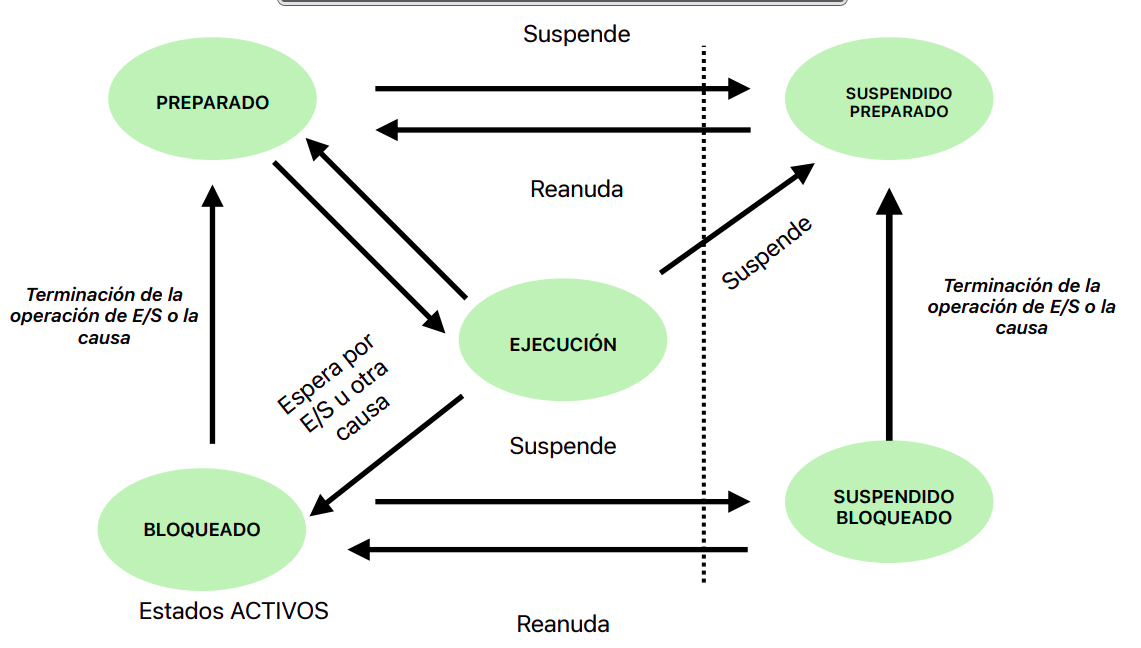
\includegraphics[width=0.8\linewidth]{Imagenes/procesosesquema.png}
	\caption{Estado de los procesos y sus transiciones. }
	\label{fig:enter-label}
\end{figure}

Los estados de los procesos se pueden dividir en dos categorías principales: \textbf{activos} e \textbf{inactivos}.

\newpage
\subsubsection{Estados activos}

Los estados activos son aquellos en los que un proceso está involucrado directamente en la ejecución o está preparado para ejecutarse. Estos estados incluyen:

\begin{tcolorbox}
\begin{itemize}
	\item \textbf{En ejecución:} El proceso está actualmente utilizando la CPU para ejecutar sus instrucciones. En este estado, el procesador está ocupado realizando las tareas definidas por el proceso. 
	
	\textbf{Ejemplo:} Si estás utilizando un editor de texto para escribir un documento, el proceso que maneja el editor de texto está en ejecución cuando estás escribiendo activamente.
	
	\item \textbf{Preparado:} El proceso está listo para ejecutarse y está esperando que el sistema operativo le asigne la CPU. Los procesos en este estado se encuentran en la cola de procesos listos. 
	
	\textbf{Ejemplo:} Si tienes varias pestañas abiertas en un navegador, los procesos que manejan las pestañas inactivas están en el estado de preparado, esperando su turno para recibir tiempo de CPU.
	
	\item \textbf{Bloqueado:} El proceso no puede continuar su ejecución hasta que se cumpla una condición externa, como la finalización de una operación de entrada/salida (E/S) o la disponibilidad de un recurso. A pesar de estar en espera, el proceso sigue siendo considerado ``activo'' porque se espera que retome la ejecución tan pronto como la condición que lo bloquea se resuelva.
	
\end{itemize}
\end{tcolorbox}

\subsubsection{Estados inactivos}

Los estados inactivos son aquellos en los que un proceso no está utilizando la CPU y ha sido suspendido temporalmente por el sistema operativo. Estos estados incluyen:

\begin{tcolorbox}
\begin{itemize}
	\item \textbf{Suspendido bloqueado:} El proceso estaba en el estado de \textit{Bloqueado} pero ha sido movido a la memoria secundaria (swap) debido a que el sistema necesita liberar espacio en la memoria principal. En este estado, el proceso no puede avanzar ni siquiera cuando se resuelve la condición que lo bloqueaba, hasta que sea devuelto a la memoria principal.
	
	
	\item \textbf{Suspendido preparado:} El proceso estaba en el estado de \textit{Preparado} y ha sido movido a la memoria secundaria. A diferencia del estado \textit{Suspendido Bloqueado}, este proceso está listo para ejecutarse tan pronto como sea devuelto a la memoria principal y reciba tiempo de CPU.

\end{itemize}

\end{tcolorbox}

La clasificación de los estados de los procesos en activos e inactivos permite al sistema operativo gestionar de manera eficiente los recursos y la ejecución de los procesos. Los estados activos indican que el proceso está participando activamente en la ejecución o está preparado para hacerlo, mientras que los estados inactivos indican que el proceso ha sido suspendido temporalmente y no está en memoria principal.

\newpage
\subsection{Transiciones de estado}
Todo proceso a lo largo de su vida puede cambiar de estado varias veces. cada uno de estos cambios se llama \textbf{transición de estado}. Estas transiciones son las siguientes:
\begin{tcolorbox}
	
	
	\begin{itemize}
		\item \subsubsection {Comienzo de la ejecución}
		Todo proceso comienza cuando se emite la orden de ejecución del programa. Inicialmente, el proceso se inserta en la \textbf{cola de preparados}. El encolamiento de procesos en esta cola dependerá de la política de gestión que utilice el sistema operativo.
		
		\item \subsubsection {Paso a estado de ejecución}
		Cuando el procesador se encuentra inactivo y en la cola de preparados existe algún proceso en espera de ser ejecutado, el primer proceso en la cola es seleccionado y se le asigna la CPU, cambiando su estado a \textbf{en ejecución}.
		
			\item \subsubsection {Paso a estado bloqueado}
		Un proceso en ejecución puede necesitar realizar una operación de entrada/salida (E/S), como leer un archivo desde el disco. En este caso, debido a que la operación de E/S puede tardar en completarse, el proceso no puede continuar ejecutándose inmediatamente. Por lo tanto, se cambia su estado a \textbf{bloqueado} y su PCB se inserta en la \textbf{cola de bloqueados}.
		
				\item \subsubsection{Paso a estado preparado}
		Un proceso puede pasar al estado preparado desde varios otros estados, bajo las siguientes circunstancias:
		
		\begin{itemize}
			\item \textbf{Orden de ejecución de un programa:} Cuando se inicia un nuevo proceso, se inserta en la cola de preparados.
			\item \textbf{Finalización de una operación de E/S:} Si un proceso estaba bloqueado esperando la finalización de una operación de E/S, una vez que la operación se completa, el proceso se mueve de la \textbf{cola de bloqueados} a la \textbf{cola de preparados}.
			\item \textbf{Interrupción del proceso en ejecución:} Si un proceso en ejecución es interrumpido (por ejemplo, por una interrupción de hardware o por el sistema operativo), su estado cambia a preparado, y su PCB se mueve a la \textbf{cola de preparados}.
			\item \textbf{Activación de un proceso suspendido:} Un proceso previamente suspendido (sin estar bloqueado) puede ser reactivado, lo que lo moverá a la cola de preparados.
		\end{itemize}
		

						\end{itemize}	
	\end{tcolorbox}	






\begin{tcolorbox}


	\begin{itemize}
		
		
	
		
	
		

	

	
		
		\item \subsubsection {Paso a estado suspendido bloqueado}
		Si un proceso está bloqueado y el sistema operativo necesita liberar memoria o suspender el proceso por alguna razón, el proceso es movido a estado \textbf{suspendido bloqueado}. Su PCB se traslada a la \textbf{cola de procesos suspendidos bloqueados}.
		
		\begin{itemize}
			\item \textbf{Ejemplo:} Un proceso que estaba esperando la respuesta de una operación de red puede ser suspendido si el sistema operativo necesita liberar recursos. 
		\end{itemize}
		
			\item \subsubsection{Paso a estado suspendido preparado} 
		Un proceso puede pasar a este estado en tres circunstancias diferentes:
		
		\begin{itemize}
			\item \textbf{Suspensión de un proceso preparado:} Un proceso en la cola de preparados puede ser suspendido, moviéndose así a la \textbf{cola de suspendidos preparados}.
			\item \textbf{Suspensión de un proceso en ejecución:} Si un proceso en ejecución es suspendido, su estado cambia a suspendido preparado, y su PCB se mueve a la cola de suspendidos preparados.
			\item \textbf{Desbloqueo de un proceso suspendido bloqueado:} Si se elimina la causa que bloqueaba un proceso suspendido bloqueado, este proceso se moverá a la cola de suspendidos preparados.
		\end{itemize}
		
	\end{itemize}
\end{tcolorbox}





\subsection{Operaciones sobre procesos}

Los sistemas operativos modernos proporcionan varias funciones para manipular y gestionar los procesos. A continuación, se describen las principales operaciones que se pueden realizar sobre un proceso:


\begin{tcolorbox}

\begin{itemize}
	\item \textbf{Crear un proceso:}
	La creación de un proceso se inicia mediante la orden de ejecución de un programa. Este proceso requiere varios argumentos, como el nombre del proceso y su prioridad. En este momento, se crea el \textbf{Bloque de Control de Procesos (PCB)}, que se inserta en la \textbf{cola de procesos preparados}.
	
	\begin{itemize}
		\item \textbf{Creación jerárquica:} En este tipo de creación, cada proceso que se crea es hijo del proceso creador y hereda el entorno de ejecución de su padre. Por ejemplo, el primer proceso que ejecuta un usuario suele ser hijo del intérprete de comandos con el que interactúa.
		\item \textbf{Creación No Jerárquica:} En esta modalidad, cada proceso creado por otro proceso se ejecuta independientemente de su creador y con un entorno diferente. Este tipo de creación no es común en los sistemas operativos modernos.
	\end{itemize}
	
	\item \textbf{Destruir un proceso:}
	La destrucción de un proceso implica la eliminación del proceso mediante una orden específica. Esta operación resulta en la eliminación del PCB asociado con el proceso.
	

	
	\end{itemize}
	
	\end{tcolorbox}
	
	
	\begin{itemize}
		
	\begin{tcolorbox}


	
	\item \textbf{Suspender un proceso:}
	La suspensión de un proceso es una operación de alta prioridad que paraliza el proceso, permitiendo que pueda ser reanudado posteriormente. Esta operación es útil en situaciones de malfuncionamiento o sobrecarga del sistema.
	

	
	\item \textbf{Reanudar un proceso:}
	La reanudación de un proceso se refiere a la activación de un proceso que ha sido previamente suspendido, permitiendo que continúe su ejecución desde el punto en el que fue interrumpido.
	

	
	\item \textbf{Cambiar la prioridad de un proceso:}
	Esta operación permite ajustar la prioridad de un proceso en ejecución, lo que puede afectar el orden en el que el proceso recibe tiempo de CPU en comparación con otros procesos.
	

	
	\item \textbf{Temporizar la ejecución de un proceso:}
	La temporización de un proceso controla su ejecución en función de un periodo de tiempo fijo, permitiendo que el proceso se ejecute en intervalos regulares o en una sola vez después de un período determinado.
	

	
	\item \textbf{Despertar un proceso:}
	Despertar un proceso se refiere a desbloquear un proceso que ha sido previamente bloqueado debido a la temporización u otras causas.
	

	
		\end{tcolorbox}
	
\end{itemize}



\subsection{Prioridades}


En un sistema operativo, cada proceso tiene asignada una prioridad que determina cómo y con qué frecuencia puede acceder al procesador en comparación con otros procesos. Esta prioridad refleja las necesidades de ejecución del proceso en cuanto a urgencia y asignación de recursos, influenciando directamente el orden y la velocidad con la que se ejecutan los procesos en el sistema.

Las prioridades se pueden clasificar de diferentes maneras, según cómo se asignan y si pueden o no modificarse durante la ejecución del proceso.




\begin{itemize}
	\item \textbf{Clasificación según la asignación de la prioridad:}
	\begin{itemize}
		\begin{tcolorbox}

	
		\item \textbf{Asignadas por el sistema operativo:}
		Estas prioridades son asignadas automáticamente por el sistema operativo en el momento en que el proceso comienza su ejecución. La asignación de estas prioridades depende principalmente de los privilegios del propietario del proceso y del modo de ejecución en el que se encuentra.
		
		\begin{itemize}
			\item \textbf{Ejemplo:} Un proceso iniciado por un administrador del sistema puede recibir una prioridad más alta que un proceso iniciado por un usuario regular.
		\end{itemize}
		
		\item \textbf{Asignadas por el propietario:}
		En este caso, es el propio usuario quien asigna la prioridad con la que un proceso debe ejecutarse. Este enfoque es común en sistemas de tiempo real, donde ciertos procesos necesitan responder rápidamente a eventos sin ser interrumpidos.
		
		\begin{itemize}
			\item \textbf{Ejemplo:} En un sistema de control industrial, un usuario podría asignar una alta prioridad a un proceso que monitorea la temperatura, asegurando que no se demore su ejecución.
		\end{itemize}
			\end{tcolorbox}
	\end{itemize}
	
	\newpage
	\item \textbf{Clasificación según la variabilidad de la prioridad:}
	\begin{itemize}
		\begin{tcolorbox}

		\item \textbf{Estáticas:}
		Las prioridades estáticas son aquellas que no pueden ser modificadas durante la ejecución del proceso. Una vez que se asigna una prioridad estática, permanece constante durante todo el ciclo de vida del proceso. Este tipo de prioridad es utilizado en sistemas de tiempo compartido, donde la equidad en la asignación de recursos es importante, pero no en sistemas de tiempo real, donde la flexibilidad y la capacidad de respuesta rápida son cruciales.
		
		\begin{itemize}
			\item \textbf{Ejemplo:} Un proceso de mantenimiento del sistema que tiene una prioridad estática podría estar programado para ejecutarse con regularidad, sin cambios en su prioridad.
		\end{itemize}
		
		\item \textbf{Dinámicas:}
		Las prioridades dinámicas pueden ser modificadas durante la ejecución del proceso. Este ajuste permite que el sistema operativo reaccione a eventos cambiantes, ajustando la prioridad de los procesos para asegurar que se manejen adecuadamente.
		
		\begin{itemize}
			\item \textbf{Ejemplo:} Si un proceso de baja prioridad requiere atención urgente debido a un evento crítico, el sistema operativo puede elevar temporalmente su prioridad para asegurar que se maneje rápidamente.
		\end{itemize}
		
		\end{tcolorbox}
	\end{itemize}
\end{itemize}

\subsection{Tipos de procesos}

Los procesos en un sistema operativo se pueden clasificar en varias categorías según diferentes criterios, como el uso que se les dará, cómo se construyó el código ejecutable, su capacidad de acceso a los recursos, y su forma de ejecución. A continuación, se describen los principales tipos de procesos:

\begin{itemize}
	
	
	
	\item \textbf{Clasificación según el uso y la construcción del código ejecutable:}
	
	

	
	\begin{itemize}
		\begin{tcolorbox}
		\item \textbf{Reutilizables:}
		Estos procesos pueden cambiar los datos que utilizan, pero si se vuelven a ejecutar, necesitan comenzar en su estado inicial y procesar nuevos datos. Este tipo de procesos es común en los programas normales del usuario.
		
		\begin{itemize} 
			\item \textbf{Ejemplo: }Un videojuego, donde un usuario nuevo genera una nueva partida.
		\end{itemize}
		
		\item \textbf{Reentrantes:}
	Los procesos reentrantes son programas que pueden ser utilizados por varios usuarios o tareas al mismo tiempo sin que se interfieran entre ellos. Esto es posible porque no guardan datos que cambien en su memoria; en lugar de eso, cada usuario o tarea tiene su propio espacio para manejar sus datos, mientras todos comparten el mismo código del programa.
		
		\begin{itemize}
			\item \textbf{Ejemplo:} Una calculadora online, permite muchos usuarios de manera "simultánea".
		\end{itemize}
	\end{tcolorbox}
	\end{itemize}
	
	\newpage
	\item \textbf{Clasificación según la capacidad de acceso a los recursos:}
	
	\begin{itemize}
		\begin{tcolorbox}
		\item \textbf{Apropiativos:}
		Los procesos apropiativos son aquellos que, una vez que tienen asignado un recurso, no permiten que otro proceso acceda a ese recurso hasta que hayan terminado de utilizarlo.
		
		\begin{itemize}
			\item \textbf{Ejemplo:} Una impresora; mientras el proceso utiliza la impresora, no permite que otro proceso pueda acceder a ella.
		\end{itemize}
		
		\item \textbf{No Apropiativos:}
		Los procesos no apropiativos permiten que otros procesos accedan a un recurso que están utilizando, lo que facilita el uso compartido de recursos entre múltiples procesos.
		
		\begin{itemize}
			\item \textbf{Ejemplo:} Un proceso que utiliza una base de datos en modo compartido es un proceso no apropiativo, ya que permite que otros procesos accedan a la misma base de datos simultáneamente.
		\end{itemize}
	\end{tcolorbox}
	\end{itemize}
	
	
	
	
	\item \textbf{Clasificación según la forma de ejecución:}
	
	\begin{itemize}
		
		\begin{tcolorbox}


		\item \textbf{Residentes:}
		Los procesos residentes son aquellos que permanecen en la memoria principal durante todo el tiempo que dure su ejecución.
		
	
		
		\item \textbf{Intercambiables:}
		Los procesos intercambiables pueden ser llevados desde la memoria principal al disco mientras están bloqueados. La memoria principal liberada por estos procesos puede ser utilizada por otros procesos que la necesiten en ese momento.
	
		
			\end{tcolorbox}
	\end{itemize}
	

	
\end{itemize}

\newpage

\subsection{Excepciones}

A lo largo de la ejecución de un proceso, pueden surgir una serie de irregularidades o fallos que el sistema operativo debe controlar y, si es posible, corregir. Estos problemas, conocidos como excepciones, pueden ser de diversa naturaleza y afectar al proceso de diferentes maneras. Entre los tipos de excepciones que pueden ocurrir, se incluyen:

\begin{itemize}
	\begin{tcolorbox}
		
	\item \textbf{Fallos de hardware:} Problemas físicos con los componentes del sistema, como fallos en la memoria o en los dispositivos de entrada/salida.
	\item \textbf{Fallos de software:} Errores en el código del programa que pueden interrumpir su correcta ejecución.
	\item \textbf{Entrada de datos incorrectos:} Datos proporcionados al programa que no cumplen con el formato o el tipo esperado.
	\item \textbf{Eventos anómalos:} Situaciones inesperadas que no se contemplaban en el diseño del programa, como la pérdida de conexión a un servidor.
	\end{tcolorbox}
\end{itemize}

Para gestionar estos eventos, los sistemas operativos incorporan lo que se denomina un \textbf{gestor de excepciones}. La misión del gestor de excepciones es controlar el software que maneja este tipo de eventos o excepciones, intentando corregirlos o, en su defecto, minimizando su impacto en el sistema.

Según la gravedad de los eventos que pueden presentarse, las excepciones se dividen en tres categorías principales:

\begin{itemize}
	\item \textbf{Errores catastróficos:} 
	Estos son errores que imposibilitan el funcionamiento del sistema operativo y no hay forma de recuperarlo. Un ejemplo de un error catastrófico sería un fallo en la tensión de alimentación del hardware, que podría provocar que el sistema se apague inesperadamente y no pueda reiniciarse correctamente.
	
	\item \textbf{Errores no recuperables:} 
	Estos errores, aunque no afectan al sistema operativo en su totalidad, impiden que el proceso afectado continúe con su ejecución. Un ejemplo típico es la aparición de una división por cero en un cálculo matemático, lo que provoca la interrupción inmediata del proceso.
	
	\item \textbf{Errores recuperables:} 
	Son errores que, con ciertos ajustes o correcciones, permiten que el proceso continúe su ejecución normal. Un ejemplo podría ser la introducción de datos en un formato incorrecto, que el sistema operativo puede corregir o solicitar nuevamente la información para evitar la interrupción del proceso.
\end{itemize}



	%\chapter{Unidad 4. Planificación del Procesador}

La planificación del procesador es una función crítica de los sistemas operativos que se encarga de gestionar cómo y cuándo los procesos reciben tiempo de CPU. Esta gestión es esencial para asegurar que todos los procesos en el sistema tengan un acceso justo y eficiente a los recursos del procesador.

\section{Niveles}
En un sistema operativo, la planificación del procesador se organiza en tres niveles principales, cada uno con un papel importante en la gestión eficiente de los recursos del sistema. Estos niveles determinan cómo y cuándo los procesos reciben acceso a la CPU.

\subsection{Planificación a largo plazo (Planificador de trabajos)}

\textbf{Función: }Este nivel de planificación se encarga de decidir qué procesos se deben admitir en el sistema. El planificador de trabajos controla la entrada de procesos nuevos en el sistema, determinando qué procesos deben ser cargados en la memoria principal para su ejecución.

En los sistemas modernos, la planificación a largo plazo es menos común, ya que los sistemas suelen tener la capacidad de manejar múltiples procesos sin necesidad de una planificación estricta a largo plazo. Sin embargo, sigue siendo relevante en sistemas con recursos limitados o en sistemas de procesamiento por lotes, donde se debe controlar la carga de trabajo.

\subsection{Planificación a Medio Plazo (Planificador de Swapping)}
\textbf{Función: }Este nivel de planificación gestiona la memoria y decide qué procesos deben ser movidos entre la memoria principal y la memoria secundaria (swap). El planificador a medio plazo es responsable de optimizar el uso de la memoria, asegurando que los procesos que necesitan más recursos estén en la memoria principal y los que están inactivos sean movidos al disco.

En los sistemas modernos, la planificación a medio plazo es crucial en la gestión de la memoria virtual. Aunque el término \textit{"swapping"} ha evolucionado, el concepto subyacente de manejar la memoria de manera eficiente sigue siendo esencial, especialmente en sistemas con un gran número de procesos activos.



\subsection{Planificación a Corto Plazo (Planificador del Procesador)}

\textbf{Función:} Este es el nivel de planificación más crítico y se encarga de decidir qué proceso en la cola de preparados debe ser ejecutado a continuación. El planificador a corto plazo realiza la conmutación de contexto y asegura que la CPU esté siempre ocupada ejecutando procesos. Lleva a cabo las funciones de la multiprogramación, estando siempre residente en memoria y ejecutándose con mucha frecuencia; estos procesos son de ejecución rápida.

\section{Objetivos}

Las políticas de planificación tienen como objetivo garantizar un uso eficiente y equitativo del procesador, además de optimizar el rendimiento general del sistema operativo. A continuación, se describen los principales objetivos que intentan cubrir estas políticas:

\subsection{Justicia}
La política de planificación debe ser justa, asegurando que todos los procesos tengan oportunidades equitativas de acceso a los recursos del sistema. Ningún proceso debe ser favorecido en detrimento de otro.

\textbf{Ejemplo:} En un sistema de tiempo compartido, todos los usuarios deben tener la misma oportunidad de acceder a la CPU sin que unos procesos monopolizen el tiempo de ejecución.

\subsection{Máxima Capacidad de Ejecución}
El objetivo es maximizar la capacidad de ejecución de la CPU, es decir, mantener el procesador ocupado el mayor tiempo posible con la menor cantidad de interrupciones. Esto se logra reduciendo el número de cambios de contexto, lo que permite que los trabajos se completen lo más rápidamente posible.

\textbf{Ejemplo:} Un algoritmo de planificación que minimiza los cambios de proceso permitirá que los trabajos se ejecuten con mayor fluidez, reduciendo el tiempo total de espera.

\subsection{Máximo Número de Usuarios Interactivos}
En sistemas de tiempo compartido, se busca que el mayor número posible de usuarios interactivos pueda trabajar simultáneamente. Esto mejora la experiencia de uso y la eficiencia en entornos multiusuario.

\textbf{Ejemplo:} En un sistema de servidores, es esencial que múltiples usuarios puedan acceder a sus aplicaciones o recursos al mismo tiempo sin que la velocidad o la respuesta se vean afectadas significativamente.

\subsection{Predecibilidad}
La política de planificación debe ser predecible, permitiendo saber cómo se ejecutarán los procesos en todo momento. Esto implica que el comportamiento del sistema sea consistente y que los procesos se ejecuten de acuerdo a las reglas establecidas.

\textbf{Ejemplo:} En un sistema crítico, como el de control de tráfico aéreo, es importante que las aplicaciones respondan de manera predecible, asegurando que las tareas críticas siempre se ejecuten en el tiempo adecuado.

\subsection{Minimización de la Sobrecarga}
El objetivo es reducir la sobrecarga del sistema. Esto incluye minimizar los cambios de contexto y las operaciones innecesarias que ralentizan el rendimiento del sistema. Cuanto menor sea la sobrecarga, mayor será la velocidad de procesamiento general del sistema.



\subsection{Equilibrio en el Uso de Recursos}
Es esencial que los recursos del sistema (CPU, memoria, dispositivos de entrada/salida) se utilicen de manera equilibrada. Esto implica que los recursos estén ocupados de manera justa y eficiente para obtener un buen rendimiento general.

\textbf{Ejemplo:} Si un proceso está utilizando demasiados recursos de E/S, el sistema operativo puede reducir su acceso a la CPU para que otros procesos tengan la oportunidad de ejecutarse.

\subsection{Seguridad de las Prioridades}
Los procesos de mayor prioridad deben recibir más atención del procesador y ejecutarse más rápidamente que aquellos con menor prioridad. Esto asegura que los procesos críticos no se vean retrasados por procesos menos importantes.

\textbf{Ejemplo:} Un proceso del sistema que gestiona la seguridad debe tener prioridad sobre los procesos de los usuarios comunes, asegurando que se ejecute sin demoras.


\section{Criterios}

Los criterios que se deben tener en cuenta a la hora de elegir o diseñar un algoritmo de planificación son los siguientes:

\subsection{Tiempo de Respuesta}
Es la velocidad con que el ordenador da respuesta a una petición. Depende principalmente de la velocidad de los dispositivos de entrada/salida (E/S), la carga del sistema y el algoritmo de planificación empleado.

\subsection{Tiempo de Servicio}
Es el tiempo total que tarda en ejecutarse un proceso. Este incluye el tiempo de carga del programa en la memoria, el tiempo de espera en la cola de procesos preparados, el tiempo de ejecución en el procesador, y el tiempo consumido en operaciones de E/S.

\subsection{Tiempo de Ejecución}
Es idéntico al tiempo de servicio, pero excluye el tiempo de espera en la cola de procesos preparados. Es el tiempo que necesitaría el proceso para completarse si fuera el único en ejecución en el sistema.

\subsection{Tiempo de Procesador}
Es el tiempo que un proceso está utilizando activamente el procesador, sin contar los periodos en los que se encuentra bloqueado, por ejemplo, debido a operaciones de E/S.

\subsection{Tiempo de Espera}
Es el tiempo en que los procesos están activos pero sin ser ejecutados, es decir, el tiempo que pasan en las colas de espera, como la cola de procesos preparados.

\subsection{Eficiencia}
La eficiencia se refiere a la utilización del procesador, el recurso más valioso en un sistema. El objetivo es que el procesador esté ocupado el mayor tiempo posible para maximizar el rendimiento, con el menor tiempo de inactividad.

\subsection{Rendimiento}
Es el número de trabajos o procesos completados por unidad de tiempo. El rendimiento óptimo se alcanza cuando el sistema es capaz de gestionar el mayor número de tareas posible en un periodo de tiempo, dependiendo del algoritmo de planificación y la carga del sistema.

\section{Medidas en la Planificación de Procesos}

Para evaluar cómo se comportan las diferentes políticas de planificación del procesador, utilizamos una serie de medidas que nos permiten analizar el rendimiento del sistema y cómo se gestionan los procesos.

\subsection{Tiempo de Servicio (T)}
El \textbf{tiempo de servicio} es el tiempo total que un proceso tarda en ejecutarse completamente desde el momento en que se da la orden de ejecución hasta que termina.

\textbf{Fórmula:} 
\[
T = t_{\text{fin}} - t_{\text{inicio}}
\]

Donde:
\begin{itemize}
	\item \( t_{\text{inicio}} \) es el momento en que el proceso comienza su ejecución.
	\item \( t_{\text{fin}} \) es el momento en que el proceso termina.
\end{itemize}

\textbf{Ejemplo:} Si un proceso comienza a ejecutarse a las 3:00 p.m. y termina a las 3:10 p.m., el tiempo de servicio sería 10 minutos.

\subsection{Tiempo de Espera (E)}
El \textbf{tiempo de espera} es el tiempo que un proceso pasa en cola, esperando a ser ejecutado. Es la diferencia entre el tiempo total del proceso y el tiempo en que realmente está usando la CPU.

\textbf{Fórmula:}
\[
E = T - t
\]

Donde:
\begin{itemize}
	\item \( T \) es el tiempo de servicio.
	\item \( t \) es el tiempo que el proceso pasa en ejecución.
\end{itemize}

\textbf{Ejemplo:} Si el tiempo total de servicio es 10 minutos, pero el proceso solo estuvo ejecutándose durante 7 minutos, el tiempo de espera sería 3 minutos.

\newpage

\subsection{Índice de Servicio (I)}
El \textbf{índice de servicio} nos indica qué tanto tiempo un proceso estuvo ejecutándose en comparación con su tiempo total en el sistema.

\textbf{Fórmula:}
\[
I = \frac{t}{T}
\]

Donde:
\begin{itemize}
	\item \( t \) es el tiempo de ejecución del proceso.
	\item \( T \) es el tiempo de servicio total.
\end{itemize}


\textbf{Interpretación:}
\begin{itemize}
	\item Un valor de \( I \) cercano a \textit{1} indica que el proceso estuvo ejecutándose la mayor parte del tiempo que estuvo en el sistema, es decir, tuvo poco tiempo de espera.
	\item Un valor de \( I \) cercano a \textit{0} indica que el proceso pasó una parte significativa de su tiempo \textbf{esperando} en cola antes de ser ejecutado.
\end{itemize}

\textbf{Ejemplo:}

Supongamos que un proceso tiene:
\begin{itemize}
	\item Tiempo de servicio total \( T = 10 \) minutos.
	\item Tiempo de ejecución \( t = 4 \) minutos.
\end{itemize}

Entonces, el Índice de Servicio sería:
\[
I = \frac{t}{T} = \frac{4 \text{ minutos}}{10 \text{ minutos}} = 0.4
\]
Esto significa que el proceso estuvo ejecutándose el **40\%** del tiempo total que estuvo en el sistema y esperando el **60\%** restante.




\subsection{Tiempo del Núcleo}
Es el tiempo que consume el núcleo del sistema operativo para tomar decisiones sobre la planificación del procesador. Este tiempo incluye los cambios de contexto, es decir, cuando el sistema guarda el estado de un proceso y carga el estado de otro para ejecutar.

\subsection{Tiempo de Inactividad (Idle)}
Es el tiempo en que la CPU no tiene ningún trabajo productivo que realizar. Esto ocurre cuando no hay procesos listos para ejecutarse, es decir, cuando la cola de procesos preparados está vacía.

\textbf{Ejemplo:} Si la computadora está encendida pero no tiene ninguna tarea que procesar, el tiempo de inactividad aumenta. Aunque el sistema sigue funcionando, la CPU está ``esperando'' por nuevas tareas.



\section{Algoritmos de planificación}

Antes de detallar los algoritmos de planificación, es importante entender las dos políticas principales que guían la planificación de los procesos:

\begin{enumerate}
	\item \textbf{Política Apropiativa:}
	En esta política, un proceso puede ser interrumpido mientras está ejecutándose y ser reemplazado por otro proceso. Esto ocurre con frecuencia cuando llega un proceso de mayor prioridad o cuando se cumple el límite de tiempo asignado al proceso en la CPU.
		
	\textbf{Ventaja:} Permite una respuesta más rápida a procesos críticos o de mayor prioridad.
	
	\textbf{Desventaja:} Genera más cambios de contexto, lo que puede aumentar la sobrecarga del sistema.
	\item \textbf{Política No Apropiativa:}
	En este caso, una vez que un proceso empieza a ejecutarse, no es interrumpido hasta que se completa. No importa si llegan procesos de mayor prioridad o más cortos durante su ejecución.
	
	\textbf{Ventaja:} Menos cambios de contexto, lo que reduce la sobrecarga del sistema.
	
	\textbf{Desventaja:} Puede hacer que procesos críticos o urgentes tengan que esperar más tiempo.
	
\end{enumerate}





\subsection{Algoritmo FCFS (First Come First Served)} El algoritmo FCFS (First Come First Served), o Primero en llegar, primero en ser atendido, es el algoritmo de planificación más simple. Los procesos son gestionados en una cola única de procesos listos, y se ejecutan en el orden en que llegan. El primer proceso en entrar a la cola será el primero en recibir el tiempo de CPU, y no será interrumpido hasta que termine su ejecución.

\textbf{Características del FCFS:}
\begin{itemize} \item Política no apropiativa: Una vez que el proceso comienza a ejecutarse, no se interrumpe hasta que se completa. \item Los procesos se ejecutan por orden de llegada: El primer proceso en llegar es el primero en ser atendido. \item Todos los procesos esperan en una sola cola: Los procesos en la cola deben esperar su turno hasta que el CPU esté libre. \end{itemize}

\begin{figure}[H] \centering 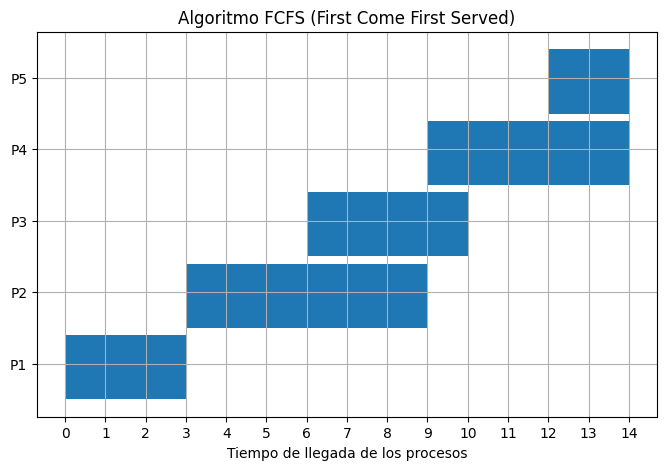
\includegraphics[width=0.8\linewidth]{Imagenes/Fcfs_tiempo.png} \caption{Se puede observar la llegada de los procesos y su tiempo de ejecución.} \end{figure}

\subsubsection{Ejecución según FCFS} Como ya se ha descrito, la ejecución de procesos mediante el algoritmo FCFS se realiza a partir de una sola cola, en orden de llegada. La llegada de un nuevo proceso lo ubicará automáticamente al final de la cola, lo que puede incrementar los tiempos de espera de los procesos más cortos que llegan después de uno largo.

\begin{figure}[H] \centering 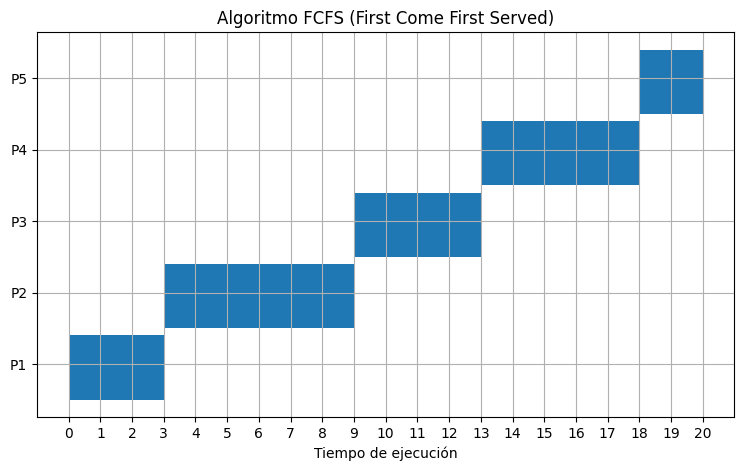
\includegraphics[width=0.8\linewidth]{Imagenes/fcfs_ejecucion.png} 
	\caption{Cola de procesos en ejecución para el algoritmo FCFS.} 
\end{figure}


\begin{itemize}
	\item P1 llega en el tiempo 0 y se ejecuta por 3 unidades de tiempo (de 0 a 3).
	\item 	P2 llega en el tiempo 3 y se ejecuta por 6 unidades de tiempo (de 3 a 9).
	\item 	P3 llega en el tiempo 6, pero espera hasta que P2 termine, y luego se ejecuta por 4 unidades de tiempo (de 9 a 13).
	\item 	
	P4 llega en el tiempo 9, pero espera hasta que P3 termine, y se ejecuta por 5 unidades de tiempo (de 13 a 18).
	\item P5 llega en el tiempo 12 y se ejecuta al final por 2 unidades de tiempo (de 18 a 20).
	
	
\end{itemize}


\subsection{Algoritmo Round Robin (RR)}

El algoritmo Round Robin (RR) es uno de los algoritmos de planificación más utilizados, especialmente en sistemas de tiempo compartido. En este algoritmo, cada proceso recibe una porción de tiempo fija, llamada cuanto de tiempo o quantum, para ejecutarse en la CPU. Si el proceso no se completa en ese tiempo, se coloca al final de la cola y se le asigna otro cuanto de tiempo en su siguiente turno. Este proceso se repite hasta que el proceso termine su ejecución.

\textbf{Características del Round Robin (RR):}
	\begin{itemize} 
		\item Política apropiativa: Si el proceso no termina dentro de su cuanto de tiempo, se interrumpe y se coloca al final de la cola de procesos listos. 
		\item Cuanto de tiempo fijo: Todos los procesos reciben la misma cantidad de tiempo para ejecutarse en cada ciclo, lo que asegura que todos los procesos reciban una oportunidad justa para usar la CPU. 
		\item Cola circular de procesos listos: Los procesos se ejecutan en orden y, si no terminan, se colocan nuevamente en la cola para su próxima oportunidad.
	\end{itemize}

\subsubsection{Ejecución según Round Robin}
	
El Round Robin es ideal para sistemas interactivos donde se necesita que todos los procesos reciban un tiempo de CPU de manera equitativa. El tamaño del cuanto de tiempo es crucial: si es muy pequeño, el sistema pasa mucho tiempo en cambios de contexto; si es muy grande, el algoritmo se comporta como FCFS.
\begin{figure}[H] \centering 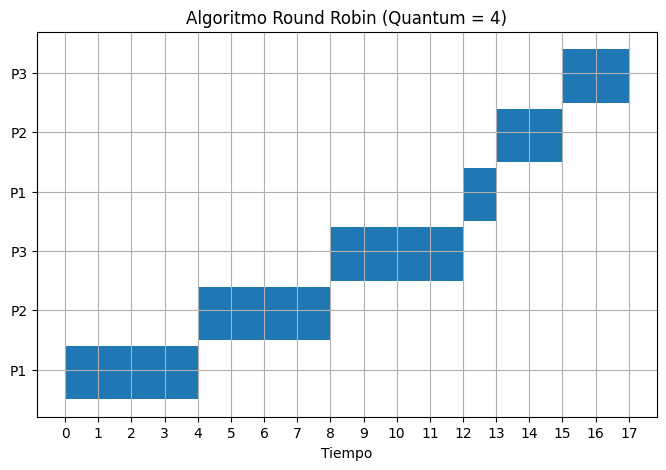
\includegraphics[width=0.8\linewidth]{Imagenes/rr_ejecucion.png} 
	\caption{Algoritmo RR en ejecución.} 
\end{figure}

\textbf{Ejemplo con \textit{quantum} de 4 unidades:}
\begin{itemize}
	\item 
	P1 tiene un tamaño 5, llega en el tiempo 0 y se ejecuta por 4 unidades de tiempo (de 0 a 4). Luego, se coloca al final de la cola.
	\item 	P2 llega con tamaño 6 y se ejecuta por 4 unidades de tiempo (de 4 a 8).
	\item 	P3 llega con tamaño 6, y se ejecuta por 4 unidades de tiempo (de 8 a 12).
	\item 	
	P1 completa su ejecución (12 a 13).
	\item P2 vuelve a ejecutarse por 2 unidades de tiempo (de 13 a 15), completando su ejecución.
	\item P3 vuelve a ejecutarse por 2 unidades de tiempo (de 17 a 17), completando su ejecución.
	
\end{itemize}

\subsection{Algoritmo SJN (Shortest Job Next)}

El algoritmo Shortest Job Next (SJN), también conocido como Shortest Process Next (SPN), selecciona el proceso con la menor duración estimada de ejecución para ser ejecutado a continuación. Es un algoritmo eficiente en términos de minimizar el tiempo promedio de espera en sistemas donde se conoce la duración de los procesos antes de que comiencen.

\textbf{Características del SJN:}
\begin{itemize} 
	\item Política no apropiativa: Una vez que el proceso con la menor duración es seleccionado, se ejecuta hasta su finalización sin interrupciones. 
	\item Minimización del tiempo promedio de espera: Como se priorizan los procesos más cortos, se optimiza el tiempo promedio de espera de todos los procesos en el sistema. \item Requiere conocimiento previo: El algoritmo necesita conocer la duración de cada proceso antes de su ejecución, lo cual puede no ser factible en algunos sistemas. \item Problema del ``hambre'': Los procesos largos pueden quedar esperando indefinidamente si continuamente llegan procesos más cortos, lo que se conoce como el problema del ``hambre'' o starvation. 
\end{itemize}

\subsubsection{Ejecución según SJN}

El algoritmo SJN selecciona siempre el proceso que tiene la menor duración para ejecutarse primero. Si varios procesos tienen la misma duración, se ejecuta el que llegó primero, similar a FCFS en este caso.

\textbf{Ejemplo:}
Supongamos que tenemos los siguientes procesos, cada uno con su tiempo de llegada y duración estimada de ejecución:

\begin{itemize} 
	\item P1 llega en el tiempo 0 y tiene una duración de 6 unidades de tiempo. 
	\item P2 llega en el tiempo 2 y tiene una duración de 4 unidades de tiempo. 
	\item P3 llega en el tiempo 4 y tiene una duración de 3 unidades de tiempo. 
	\item P4 llega en el tiempo 6 y tiene una duración de 2 unidades de tiempo. 
	\item P5 llega en el tiempo 8 y tiene una duración de 1 unidad de tiempo. 
\end{itemize}


	
	%\chapter{Proceso Paralelo e Interbloqueo}

Un concepto clave en los sistemas operativos es la aplicación de técnicas y algoritmos que optimizan la eficiencia de sus componentes, proporcionando al usuario el máximo rendimiento posible en un sistema informático. La evolución constante de las capacidades del hardware ha permitido la creación de equipos más potentes, capaces de realizar tareas en menos tiempo. Para gestionar de manera eficiente estas capacidades, las técnicas y algoritmos deben ser capaces de manejar adecuadamente las solicitudes de los procesos, tanto en el uso de dispositivos de entrada/salida como en el tiempo de procesador. Con el avance del hardware, estas solicitudes se han multiplicado, haciendo más necesario que nunca un control eficiente de los recursos.

\textbf{La analogía de los 5 filósofos}

Imaginemos cinco filósofos sentados alrededor de una mesa, cada uno con un plato de comida y un palillo a su derecha. Para comer, cada filósofo necesita dos palillos, lo que implica que deben compartir los palillos con sus vecinos. Si todos intentan comer al mismo tiempo, ninguno puede hacerlo, ya que falta un palillo para cada uno. Este escenario refleja los desafíos de la competencia entre procesos y la necesidad de coordinación para acceder a recursos compartidos.

\begin{figure}[H] \centering 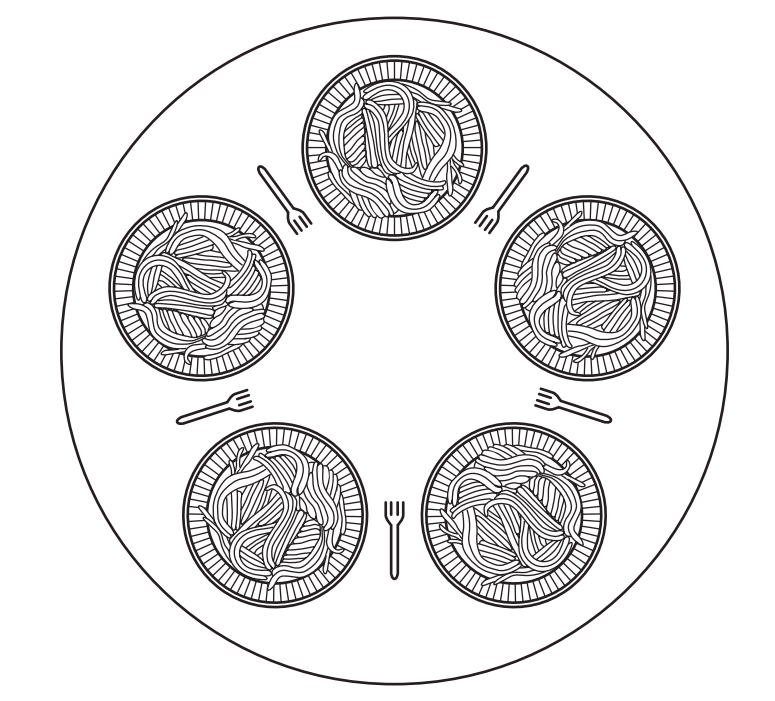
\includegraphics[width=0.8\linewidth]{Imagenes/los5filosofos.png} \caption{El problema representa los desafíos que tienen los sistemas operativos para gestionar los procesos.} \end{figure}

\section{Proceso Paralelo}

El proceso paralelo consiste en la ejecución simultánea de múltiples procesos en un sistema operativo. Su principal objetivo es mejorar el rendimiento y la eficiencia del sistema al distribuir tareas entre varios procesadores o núcleos, permitiendo que el sistema ejecute varias tareas a la vez. En sistemas con múltiples procesadores, el paralelismo es real; en sistemas de un solo procesador, el paralelismo es aparente y depende de técnicas como la multiprogramación.

El proceso paralelo es esencial para reducir tiempos de espera, aumentar la capacidad de respuesta del sistema y mejorar la experiencia del usuario. Se utiliza en aplicaciones que manejan grandes volúmenes de datos, simulaciones científicas, o en servidores que requieren alta capacidad de procesamiento.

\subsection{Exclusión Mutua}

La exclusión mutua es un principio fundamental que asegura que solo un proceso a la vez pueda acceder a un recurso compartido. Esto es importante para evitar que múltiples procesos intenten modificar el mismo recurso simultáneamente, lo que podría causar errores o corrupción de datos.

Un ejemplo claro de la necesidad de exclusión mutua ocurre en un sistema bancario. Imagina que dos cajeros automáticos, ubicados en diferentes lugares, intentan acceder al saldo de la misma cuenta bancaria para procesar retiros simultáneamente. Sin un mecanismo de exclusión mutua, ambos cajeros podrían retirar dinero al mismo tiempo, lo que provocaría que el saldo sea incorrecto o incluso que se retire más dinero del disponible. La exclusión mutua garantiza que solo uno de los cajeros pueda acceder a la cuenta en un momento dado, bloqueando temporalmente el acceso del otro hasta que la operación haya finalizado. Esto asegura que las transacciones se realicen de manera segura y consistente.

\begin{figure}[H] \centering 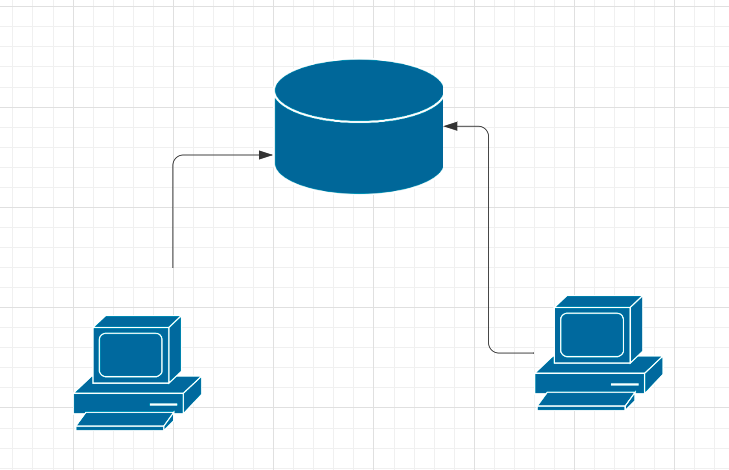
\includegraphics[width=0.8\linewidth]{Imagenes/exclusion.png} \caption{La exclusión mutua asegura que los recursos compartidos sean utilizados de manera controlada.} \end{figure}

\subsection{Sincronización}

La sincronización es el mecanismo que coordina la ejecución de múltiples procesos para asegurar que accedan a los recursos compartidos de manera ordenada y controlada. Sin la sincronización adecuada, los procesos podrían acceder a los recursos de forma desorganizada, lo que podría generar conflictos, errores o resultados inesperados.

Volviendo al ejemplo de los cajeros automáticos, la sincronización asegura que los procesos que intentan acceder al saldo de una cuenta se coordinen correctamente. Aunque la exclusión mutua previene que ambos cajeros accedan simultáneamente al saldo, la sincronización es lo que garantiza que los cajeros se coordinen y esperen su turno de manera ordenada. De esta forma, cuando un cajero completa su transacción, el otro puede acceder al saldo sin causar inconsistencias en la cuenta.

\subsubsection{Importancia de la Sincronización} \begin{itemize} \item \textbf{Integridad de Datos:} Previene condiciones de carrera, donde los resultados dependen del orden no controlado de ejecución de los procesos. \item \textbf{Eficiencia:} Permite que los procesos avancen de manera ordenada y se eviten bloqueos innecesarios, garantizando un uso óptimo de los recursos. \item \textbf{Estabilidad del Sistema:} Asegura que los procesos concurrentes no generen errores o comportamientos inesperados en el sistema operativo. \end{itemize}

\newpage

\section{Interbloqueo en Sistemas Operativos}

El \textbf{interbloqueo} es una situación en sistemas operativos donde un conjunto de procesos se encuentra en un estado de espera permanente, ya que cada uno está esperando que ocurra un evento que solo puede ser provocado por otro proceso del conjunto. Ninguno de los procesos puede avanzar porque todos dependen mutuamente de recursos que están siendo utilizados por los demás, entrando así en una espera indefinida.

\textbf{Ejemplo Ilustrativo}

Imagine una carretera de doble sentido que, en cierto punto, se estrecha debido a un puente que solo permite el paso de vehículos en un solo sentido. Si un vehículo entra desde cada extremo al mismo tiempo, ambos se encontrarán en el centro del puente. Ninguno puede avanzar porque el camino está bloqueado por el otro, y retroceder podría ser difícil o imposible. Ambos conductores esperan que el otro ceda el paso, pero si ninguno lo hace, se genera un \textbf{interbloqueo} y ambos vehículos quedan inmovilizados.

\begin{figure}[H] \centering 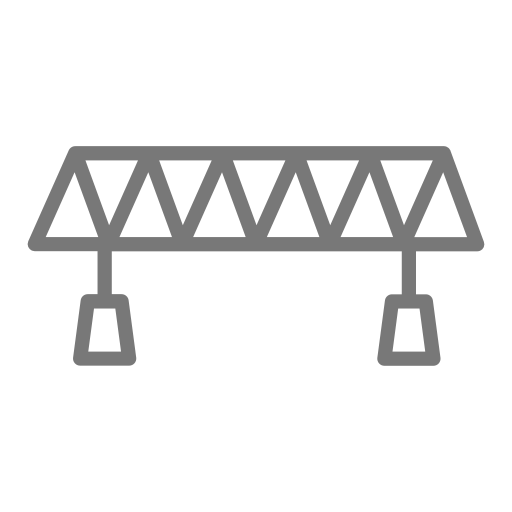
\includegraphics[width=0.6\linewidth]{Imagenes/puente.png} \caption{Un puente de una sola vía, representa al interbloqueo, cuando dos vehículos en dirección opuesta tratan de cruzar al mismo tiempo.} \end{figure}

Este ejemplo refleja cómo en un sistema operativo, procesos pueden quedar bloqueados esperando recursos que están siendo utilizados por otros procesos, sin posibilidad de que ninguno avance.

\subsection{Recursos en Sistemas Operativos}


En sistemas operativos, un \textbf{recurso} es cualquier componente de hardware o software necesario para que un proceso pueda ejecutar sus tareas. Los recursos pueden clasificarse en:
\textbf{Hardware} (CPU, Memoria, Dispositivos E/S), y \textbf{Software} (Archivos, registros). 

Estos  tienen definido un ciclo de uso, como se detalla a continuación:


\begin{enumerate}
	\item \textbf{Solicitud}: El proceso pide el recurso que necesita para continuar su ejecución.
	\item \textbf{Asignación/Utilización}: Si el recurso está disponible, el sistema operativo lo asigna al proceso, que entonces lo utiliza para realizar su tarea.
	\item \textbf{Liberación}: Una vez que el proceso ha terminado de usar el recurso, lo libera para que otros procesos puedan utilizarlo.
\end{enumerate}

Es fundamental que este ciclo se gestione de manera eficiente para evitar conflictos y asegurar que los recursos se utilizan de forma óptima.

\subsection{Modelo de Interbloqueo (Abrazo Mortal)}

El \textbf{interbloqueo}, también conocido como ``abrazo mortal'',  se produce cuando un conjunto de procesos compite por recursos y terminan bloqueándose mutuamente. Esto ocurre porque cada proceso espera que ocurra un evento (como la liberación de un recurso) que solo puede ser provocado por otro proceso dentro del mismo conjunto.

\subsubsection{¿En Qué Consiste?}

\begin{itemize}
	\item \textbf{Dependencia Circular}: Cada proceso en el conjunto está esperando por un recurso que está siendo retenido por otro proceso. Esta cadena de dependencias forma un ciclo cerrado.
	\item \textbf{Espera Indefinida}: Ninguno de los procesos puede avanzar porque están esperando indefinidamente que los recursos sean liberados, pero esto no ocurre porque todos están bloqueados.
\end{itemize}

\textbf{Ejemplo Detallado}:

Supongamos que tenemos dos procesos, \textbf{P1} y \textbf{P2}, y dos recursos, \textbf{R1} y \textbf{R2}.

\begin{itemize}
	\item \textbf{P1} tiene asignado \textbf{R1} y solicita \textbf{R2}.
	\item \textbf{P2} tiene asignado \textbf{R2} y solicita \textbf{R1}.
\end{itemize}

Ambos procesos esperan indefinidamente porque ninguno liberará su recurso hasta obtener el otro. Este es un ciclo de espera circular que provoca un interbloqueo.

\subsection{Postergación Indefinida (Starvation)}

La \textbf{postergación indefinida} ocurre cuando un proceso espera por un recurso durante un tiempo extremadamente largo o potencialmente infinito, sin garantías de que lo obtendrá. Esto suele deberse a políticas de planificación que no aseguran equidad entre los procesos.

\subsubsection{Relación con la Planificación}

\begin{itemize}
	\item \textbf{Prioridades Desbalanceadas}: Si los procesos de alta prioridad siguen llegando al sistema, los de baja prioridad pueden quedar postergados indefinidamente.
	\item \textbf{Ausencia de Mecanismos de Equidad}: Sin técnicas como la planificación circular (round-robin) o la asignación de cuotas de tiempo, algunos procesos pueden no recibir nunca los recursos que necesitan.
\end{itemize}

Aunque la postergación indefinida y el interbloqueo pueden parecer similares porque ambos resultan en procesos que no avanzan, son problemas distintos. En la postergación indefinida, no hay dependencia cíclica de recursos; es un problema de planificación y asignación de recursos.

\subsection{Condiciones para el Interbloqueo}

Para que ocurra un interbloqueo, deben cumplirse simultáneamente las siguientes cuatro condiciones:

\begin{enumerate}
	\item \textbf{Exclusión Mutua}: Mecanismo por el cual se garantiza que solo un proceso a la vez pueda acceder a un recurso. Por ejemplo, una impresora.
	\item \textbf{Posesión y Espera}: Un proceso está sosteniendo al menos un recurso y está esperando para obtener recursos adicionales que están siendo sostenidos por otros procesos. Por ejemplo, un proceso tiene una impresora y espera por un escáner que está en uso.
	\item \textbf{No Apropiación}: Los recursos no pueden ser retirados forzosamente de los procesos que los poseen; solo pueden ser liberados voluntariamente. Esto significa que si un proceso sostiene un recurso y otro proceso necesita ese mismo recurso, el sistema no puede forzar al proceso que lo tiene a liberar dicho recurso. 
	\item \textbf{Espera Circular}: Existe un conjunto de procesos \(\{P_1, P_2, \ldots, P_n\}\) tal que \(P_1\) está esperando un recurso sostenido por \(P_2\), \(P_2\) está esperando un recurso sostenido por \(P_3\), \ldots, y \(P_n\) está esperando un recurso sostenido por \(P_1\).
\end{enumerate}

Si todas estas condiciones se cumplen al mismo tiempo, el sistema está en un estado de interbloqueo.

\subsection{Tratamiento del Interbloqueo}

Existen varias estrategias para manejar los interbloqueos en sistemas operativos:

\subsubsection{1. Ignorar el Problema}

\begin{itemize}
	\item \textbf{Política del ``Ostrich''}: El sistema asume que los interbloqueos son tan poco frecuentes que no vale la pena invertir en mecanismos para prevenirlos o resolverlos.
	\item \textbf{Ventajas}:
	\begin{itemize}
		\item Simplicidad en el diseño del sistema operativo.
		\item Ahorro de recursos y tiempo de procesamiento.
	\end{itemize}
	\item \textbf{Desventajas}:
	\begin{itemize}
		\item Riesgo de que el sistema se congele si ocurre un interbloqueo.
		\item No es adecuado para sistemas donde la confiabilidad es crítica.
	\end{itemize}
\end{itemize}

\subsubsection{2. Prevención del Interbloqueo}

Esta estrategia modifica el sistema para garantizar que al menos una de las condiciones necesarias para el interbloqueo no pueda ocurrir.

\begin{itemize}
	\item \textbf{Eliminar la Exclusión Mutua}:
	\begin{itemize}
		\item Difícil, ya que algunos recursos son inherentemente no compartibles.
		\item Solución: Diseñar recursos virtuales o utilizar mecanismos de spooling (por ejemplo, en impresoras).
	\end{itemize}
	\item \textbf{Evitar la Posesión y Espera}:
	\begin{itemize}
		\item Requerir que los procesos soliciten todos los recursos que necesitan al inicio.
		\item Desventaja: Ineficiente y puede conducir a la subutilización de recursos.
	\end{itemize}
	\item \textbf{Permitir la Apropiación}:
	\begin{itemize}
		\item Si un proceso necesita un recurso, el sistema puede quitarle el recurso a otro proceso.
		\item Implementado mediante mecanismos de suspensión y reanudación de procesos.
	\end{itemize}
	\item \textbf{Romper la Espera Circular}:
	\begin{itemize}
		\item Impone un orden jerárquico en la solicitud de recursos.
		\item Los procesos deben solicitar recursos en un orden predefinido.
	\end{itemize}
\end{itemize}



\subsubsection{4. Detección y Recuperación}

Permitir que el interbloqueo ocurra, pero tener mecanismos para detectarlo y recuperarse.

\begin{itemize}
	\item \textbf{Detección}:
	\begin{itemize}
		\item Implementar algoritmos que periódicamente verifican si el sistema está en un estado de interbloqueo.
		\item Buscan ciclos en el \textit{grafo de asignación de recursos}.
	\end{itemize}
	\item \textbf{Recuperación}:
	\begin{itemize}
		\item \textbf{Abortar Procesos}: Terminar uno o más procesos para romper el ciclo de espera.
		\begin{itemize}
			\item Criterios: Prioridad del proceso, tiempo de ejecución, recursos utilizados.
		\end{itemize}
		\item \textbf{Reclamo forzado	 de Recursos}: Forzar la liberación de recursos de ciertos procesos.
		\begin{itemize}
			\item Puede requerir la implementación de puntos de recuperación (checkpoints) para reiniciar procesos.
		\end{itemize}
	\end{itemize}
\end{itemize}




		
	%\chapter{Unidad 6. Gestión de la memoria principal}
La memoria principal, o memoria RAM (Random Access Memory), es un componente esencial en los sistemas informáticos. 
Almacena temporalmente los datos y programas que están en ejecución o listos para ser ejecutados por la CPU (Unidad Central de Procesamiento). A diferencia de la memoria secundaria, la memoria principal permite un acceso rápido y directo, lo cual es crucial para el rendimiento y eficiencia del sistema.
\section{
	Direccionamiento
}
El direccionamiento se refiere al proceso mediante el cual el sistema operativo y el hardware de la computadora determinan y gestionan las ubicaciones de memoria donde se almacenan los datos e instrucciones. Este proceso involucra la asignación y la manipulación de direcciones de memoria que se utilizan para acceder a los datos que un proceso necesita durante su ejecución.

Existen \textbf{dos tipos de direccionamiento:}
\begin{itemize}
	\item \textbf{Direccionamiento físico:} Corresponden a ubicaciones reales en la memoria RAM. Son las direcciones que utiliza el hardware para acceder a los datos almacenados.
	\item \textbf{Direccionamiento lógico:} Son generadas por la CPU y utilizadas por los programas en ejecución. Representan una abstracción de la memoria física y permiten que cada proceso tenga su propio espacio de direcciones.
\end{itemize}
\begin{figure}[H] \centering 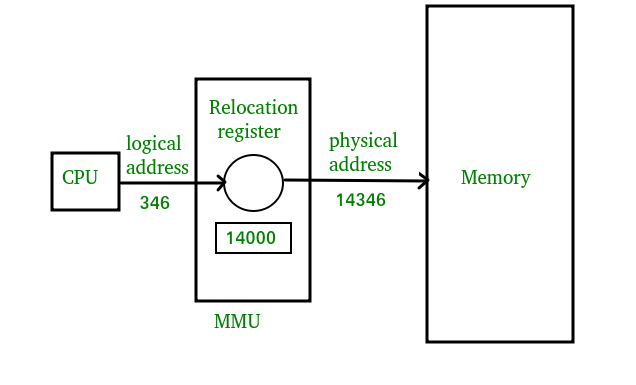
\includegraphics[width=0.6\linewidth]{Imagenes/direccionamiento.png} \caption{El procesador genera direcciones lógicas, mientras que la memoria RAM, contiene direcciones físicas.} \end{figure}

\subsection{Asignación de direcciones por MMU}

En el contexto de la gestión de la memoria principal, el direccionamiento se refiere al proceso mediante el cual el sistema operativo y el hardware de la computadora determinan y gestionan las ubicaciones de memoria donde se almacenan los datos e instrucciones. Este proceso involucra la asignación y la manipulación de direcciones de memoria que se utilizan para acceder a los datos que un proceso necesita durante su ejecución.

\begin{figure}[H] \centering 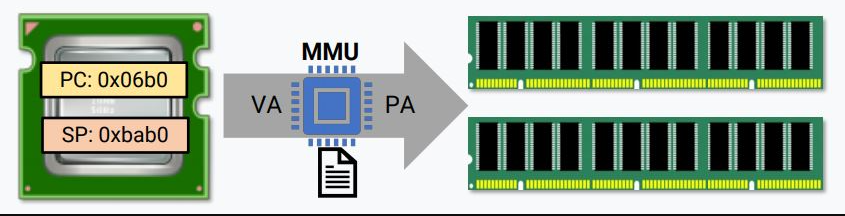
\includegraphics[width=0.6\linewidth]{Imagenes/mmu.png} \caption{La unidad MMU gestiona las ubicaciones de memoria.} \end{figure}


 \section{Jerarquía de almacenamiento}
La jerarquía de almacenamiento es un modelo que organiza los distintos tipos de memoria en un sistema computacional, incluyendo tanto la memoria volátil (RAM, caché, registros) como la memoria no volátil (discos duros, SSD), en niveles jerárquicos. Se basa en tres criterios principales: velocidad, costo y capacidad. Cada nivel de la jerarquía tiene características diferentes, con las memorias más cercanas a la CPU siendo más rápidas pero más costosas y de menor capacidad, mientras que las me

\begin{figure}[H] \centering 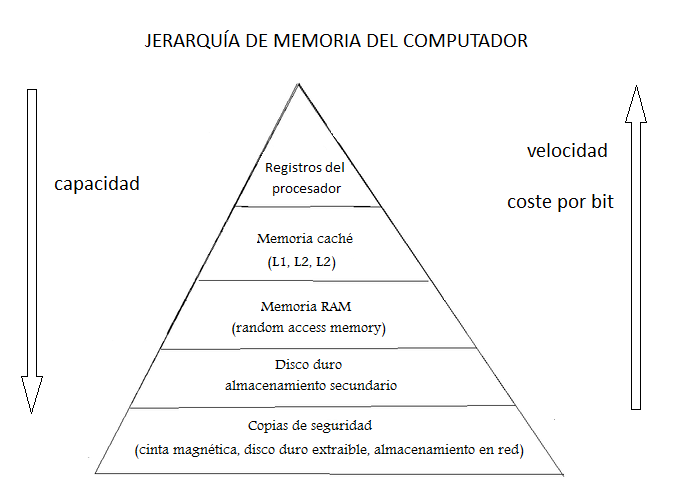
\includegraphics[width=0.6\linewidth]{Imagenes/coste.png} \caption{En la jerarquía de almacenamiento,  la capacidad es inversamente proporcional  a la velocidad y coste.} \end{figure}

\subsection{Niveles de jerarquía de almacenamiento}
En la figura anterior se muestran los diferentes niveles de la jerarquía de almacenamiento. A medida que se asciende en la pirámide, se aumenta la velocidad de acceso, pero se reduce la capacidad y el costo por bit es mayor. A continuación se describe cada nivel de manera detallada:


 \begin{tcolorbox}[title= Níveles de almacenamiento]
	\begin{itemize}
		
		
		\item \textbf{Registros:}
		Los registros están ubicados dentro del núcleo del CPU. Son la memoria más cercana al procesador, con capacidad muy limitada (solo unos pocos bytes), pero su acceso es el más rápido de todo el sistema. Los registros se utilizan para almacenar datos temporales y resultados inmediatos que se requieren para ejecutar instrucciones rápidamente.
		\item \textbf{Memoria caché:}
		La memoria caché también está ubicada dentro del procesador y se organiza en varios niveles: L1, L2 y L3. La caché L1 es la más rápida y cercana al núcleo del procesador, pero también la más pequeña. La caché L2 es más grande y ligeramente más lenta, mientras que la caché L3 es compartida entre todos los núcleos de la CPU, permitiendo que la comunicación entre estos sea más eficiente. La memoria caché almacena datos e instrucciones que se utilizan con frecuencia, reduciendo así la necesidad de acceder a la memoria RAM.
		\item \textbf{Memoria RAM:}
		La memoria RAM es la memoria volátil donde se cargan los programas y datos que están siendo utilizados activamente por el sistema. Aunque la RAM ha alcanzado grandes capacidades de almacenamiento en los sistemas modernos, su contenido se pierde cuando el equipo se apaga. Es más lenta que la caché, pero mucho más rápida que el almacenamiento secundario, y es esencial para la ejecución eficiente de programas.
		\item \textbf{Almacenamiento Secundario:}
		El almacenamiento secundario incluye dispositivos como discos duros (HDD) y unidades de estado sólido (SSD), que se utilizan para almacenar datos y programas de manera permanente. Los discos duros tradicionales (HDD) son más lentos y más baratos por bit, pero ofrecen grandes capacidades de almacenamiento. Las SSD, aunque más rápidas, son más costosas por bit y suelen tener capacidades menores en comparación con los HDD. El acceso a esta memoria es mucho más lento que en la RAM, pero su gran capacidad la hace ideal para almacenar grandes volúmenes de datos.
		
	\end{itemize}
\end{tcolorbox}



\section{Gestión de la memoria}
La gestión de la memoria es una función del sistema operativo que administra la memoria principal (RAM). Podemos establecer que el gestor de memoria:

\begin{itemize}
	\item Asigna y libera memoria a los procesos.
	\item Hace un seguimiento sobre el uso de la memoria para evitar conflictos.
	\item Optimiza el rendimiento asegurando el uso eficiente de la memoria.
\end{itemize}

El gestor de memoria es fundamental para garantizar un uso adecuado de la memoria, proporcionando una base sólida para las distintas técnicas de gestión que permiten la coexistencia de procesos en la memoria principal.

Para optimizar la gestión de la memoria, se utilizan técnicas como la monoprogramación y la multiprogramación, que permiten administrar de manera más eficiente el uso de la memoria según las necesidades del sistema.

\subsection{Monoprogramación}
La monoprogramación permite ejecutar un solo proceso a la vez. Toda la memoria principal se asigna al proceso en ejecución.

\begin{itemize}
	\item \textbf{Memoria dedicada: }Toda la memoria se asigna a un único proceso, sin interferencias. Esto es simple, pero ineficiente si el proceso no usa toda la memoria.
	\item \textbf{Monitor residente: }Parte del sistema operativo siempre reside en la memoria para gestionar tareas básicas, lo que reduce la memoria disponible para el proceso.
\end{itemize}

\textbf{Ventajas}: Simplicidad y fácil gestión.

\textbf{Desventajas}: Uso ineficiente del CPU y la memoria, ya que solo se ejecuta un proceso a la vez.

\subsection{Multiprogramación}
 La multiprogramación permite que varios procesos residan en la memoria al mismo tiempo, maximizando el uso del CPU.
 
 \begin{itemize}
 
 	\item \textbf{Particiones de la memoria:}
 	\begin{itemize}
 		\item\textbf{ Fijas: }Se dividen en secciones de tamaño fijo. Es simple, pero puede generar fragmentación interna.
 		\item \textbf{Variables: }Se ajustan al tamaño del proceso. Reducen la fragmentación interna, pero pueden generar fragmentación externa.
 	\end{itemize}
 		\item \textbf{Protección de la memoria: }Cada proceso tiene acceso solo a su propia porción de memoria, garantizado por registros de base y límite que son verificados por la MMU.
 	\item \textbf{Algoritmos de asignación:}
 	\begin{itemize}
 		\item First-Fit: Asigna la primera porción libre suficientemente grande.
 		\item Best-Fit: Asigna la porción más cercana al tamaño solicitado.
 		\item Worst-Fit: Asigna la mayor porción libre disponible.
 	\end{itemize}
 \end{itemize}
 
 \textbf{Ventajas}: Mejora la utilización del CPU al ejecutar múltiples procesos. La CPU cambia a otro proceso cuando uno está en espera.
 

 
 
 
\subsection{Segmentación}

La segmentación es una técnica de gestión de la memoria que se enfoca en el punto de vista del usuario. En lugar de dividir la memoria en particiones físicas arbitrarias, la segmentación la divide en segmentos lógicos, cada uno de los cuales corresponde a una parte específica del programa o a un tipo de dato, como el código, la pila o las variables globales.

\begin{figure}[H] \centering 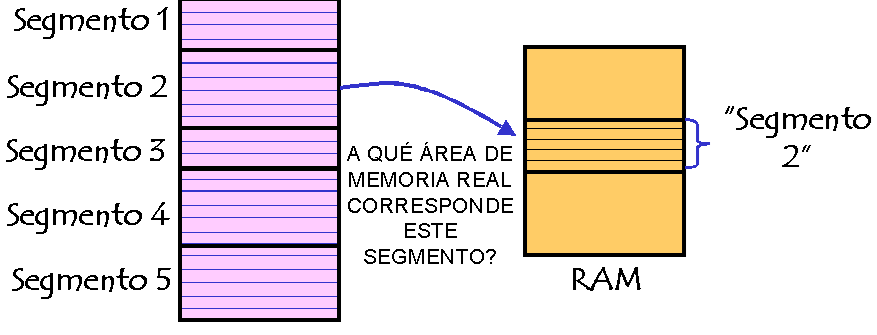
\includegraphics[width=0.6\linewidth]{Imagenes/segmentacion.png} \caption{Esquema de segmentación]} \end{figure}


\begin{itemize}
	\item Segmentos Lógicos: Cada programa se divide en segmentos lógicos, como el código, la pila, y las variables globales. Cada segmento tiene una función específica, lo que facilita la gestión de la memoria desde una perspectiva más intuitiva para el usuario.
	\item Tabla de Segmentos: El sistema operativo mantiene una tabla de segmentos para cada proceso. Esta tabla almacena la dirección base y el tamaño de cada segmento, que se utilizan para traducir las direcciones lógicas a físicas.
	\item Ventaja para el Usuario: La segmentación permite mayor flexibilidad al gestionar las diferentes partes del programa de manera independiente. Además, facilita la protección de la memoria, ya que cada segmento puede tener permisos de acceso específicos.
\end{itemize}

	


 \subsection{Memoria Virtual}
La memoria virtual es una técnica avanzada que permite a los sistemas operativos ejecutar programas que requieren más memoria de la que está físicamente disponible en la RAM. Esta técnica combina la memoria principal (RAM) con el almacenamiento secundario (disco duro o SSD) para crear una "memoria extendida" que da la impresión de tener una gran cantidad de memoria disponible.

\begin{itemize}

	
	\item \textbf{Swapping}: Cuando la memoria principal está llena, el sistema operativo utiliza el  \textbf{swapping} para intercambiar páginas activas de la RAM con páginas almacenadas en el disco. Esto permite liberar espacio en la memoria principal para otros procesos.
	
\end{itemize}
 	
		\chapter{Unidad 7. Gestión de entrada / salida (I/O)}
La gestión de entrada y salida (I/O) es una función crucial en los sistemas operativos, que facilita la interacción entre los programas y los dispositivos externos (como discos duros, teclados, monitores, impresoras, etc.). Los dispositivos periféricos necesitan intercambiar datos con la memoria y el procesador, pero no es fácil ni práctico que los procesos trabajen directamente con estos dispositivos. Afortunadamente, el sistema operativo se encarga de esta compleja tarea, actuando como intermediario para que los procesos no tengan que preocuparse por los detalles específicos de cada dispositivo. Gracias a esta gestión, los procesos pueden comunicarse con los dispositivos de manera uniforme y sin complicaciones. La entrada y salida permite que los programas realicen operaciones básicas de lectura y escritura, así como la transferencia de datos entre dispositivos de hardware y el sistema de procesamiento. El objetivo principal de la gestión de I/O es asegurar que los dispositivos de hardware funcionen de manera eficiente y que el sistema operativo gestione de forma adecuada las solicitudes de entrada y salida de múltiples procesos simultáneamente.

\textbf{Ejemplo:}
\begin{figure}[H] \centering 
\includegraphics[width=0.7\linewidth]{Imagenes/e-s.png} \caption{Al escribir, se producen varias acciones gestionadas por el controlador I/O} \end{figure}
Un ejemplo común de la importancia de la I/O es cuando un usuario escribe en un teclado (entrada) y el texto aparece en la pantalla (salida). Cuando se presiona una tecla, el teclado envía una señal al sistema operativo, que primero interpreta esta señal como un código correspondiente al carácter pulsado. Luego, el sistema operativo organiza los recursos necesarios para trasladar esta información a la memoria y notificar a la CPU. A través del controlador de video, el sistema operativo envía la información al monitor, donde finalmente el carácter se muestra en la pantalla. 
\section{Dispositivos Hardware}
Los dispositivos hardware son componentes físicos que realizan tareas de entrada y salida. Se dividen en tres grandes grupos:

\begin{tcolorbox}[title= División de los dispositivos \textit{hardware}]
	\begin{itemize}
		
		
		\item \textbf{Dispositivos de almacenamiento:}
		Estos dispositivos se encargan de guardar información, lo cual incluye discos duros, unidades de estado sólido (SSD), y discos ópticos. Son fundamentales para almacenar y recuperar datos de manera permanente o temporal.
		\item \textbf{Terminales:}
		Son dispositivos que permiten la interacción directa entre el usuario y el sistema, como teclados, pantallas y ratones. Facilitan la entrada de datos al sistema y la visualización o salida de información hacia el usuario.
		\item \textbf{Dispositivos de comunicación:}
		Incluyen tarjetas de red, módems, dispositivos WiFi, Bluetooth y otros dispositivos que permiten la transmisión de datos entre computadoras o redes. Estos dispositivos posibilitan la comunicación entre diferentes sistemas o componentes, asegurando que los datos puedan ser compartidos de forma eficiente.

		
	\end{itemize}
\end{tcolorbox}
\subsection{Tipos de dispositivos de I/O}
Los dispositivos de entrada y salida pueden clasificarse en tres tipos de acuerdo a la funcionalidad que tienen:
\begin{itemize}
	\item  \textbf{Dispositivos de entrada: }Permiten al sistema recibir datos. Ejemplos: teclados, micrófonos, cámaras.
	\item \textbf{Dispositivos de salida: }Permiten al sistema enviar datos. Ejemplos: monitores, impresoras, altavoces.
	\item  \textbf{Dispositivos de entrada/salida (I/O): }Pueden tanto recibir como enviar datos. Ejemplos: discos duros, unidades USB, tarjetas de red.
\end{itemize}
\newpage
\section{Interfaz Procesador-Periférico}
La interfaz entre el procesador y los dispositivos periféricos es esencial para la gestión de las operaciones de entrada y salida. Esta interfaz permite que los dispositivos periféricos se conecten al sistema y puedan intercambiar información con el procesador de manera eficiente. Existen tres tipos principales de conexión que facilitan esta interacción:

\begin{tcolorbox}[title= Tipos de conexión]
	\begin{itemize}
		
		
		\item \textbf{Registros:}
	Los registros son áreas de almacenamiento de alta velocidad dentro del hardware que permiten una comunicación directa entre la CPU y los dispositivos periféricos. A través de los registros, la CPU puede enviar instrucciones o datos a un periférico y recibir respuestas rápidamente. Por ejemplo, cuando se escribe un carácter con el teclado, este se almacena temporalmente en un registro antes de ser procesado.
	\item \textbf{Controladores:}
	Los controladores, también conocidos como adaptadores o interfaces de dispositivos, son circuitos o chips dedicados que actúan como intermediarios entre la CPU y los dispositivos periféricos. Estos componentes permiten que la CPU delegue tareas específicas a los periféricos. Los controladores traducen las instrucciones de la CPU a un lenguaje que el dispositivo puede entender y gestionan señales como interrupciones para informar a la CPU cuando una tarea ha sido completada. Un ejemplo común es el controlador de una impresora, que recibe datos de la CPU y controla la impresora para que realice la impresión.
	\item \textbf{Canales:}
	Los canales son mecanismos más complejos y avanzados que los registros y controladores. Se utilizan para gestionar transferencias de datos de gran volumen entre la CPU y los dispositivos periféricos. Los canales pueden operar de manera semi-independiente, lo que significa que permiten transferir datos sin la constante supervisión de la CPU, liberándola para que realice otras tareas. Esto es particularmente útil en operaciones que implican grandes volúmenes de datos, como la transferencia de archivos desde un disco duro a la memoria principal. Un ejemplo típico es el uso de canales DMA (Acceso Directo a Memoria), que gestionan grandes transferencias de datos con mínima intervención de la CPU. Algunos dispositivos gráficos modernos también utilizan DMA para enviar datos directamente a la pantalla, sin la intervención constante de la CPU.
	
		
	\end{itemize}
\end{tcolorbox}


\newpage

\section{Terminales}
Las terminales son dispositivos que combinan un teclado y una pantalla, permitiendo la interacción directa del usuario con el sistema. Las terminales son fundamentales para el ingreso y visualización de información en tiempo real. Existen diferentes tipos de terminales, según la forma en la que se conectan y operan:
\begin{tcolorbox}[title= Categorias de terminales]
	\begin{itemize}
		
		
		\item \textbf{Terminales RS-232:}
		Estas terminales se conectan a través del estándar de comunicación RS-232, que es un protocolo serial ampliamente utilizado para la transmisión de datos entre computadoras y periféricos. Este tipo de conexión es común en dispositivos antiguos, como terminales de texto, impresoras y algunos módems. A pesar de que ha sido reemplazado en gran medida por interfaces más rápidas, el RS-232 aún se usa en aplicaciones industriales y sistemas embebidos debido a su simplicidad y fiabilidad. Un ejemplo son los sistemas de inventario en almacenes, que aún utilizan RS-232 debido a la estabilidad del protocolo.
		\item \textbf{Terminales mapeadas en memoria:}
		Son terminales cuya pantalla está directamente vinculada a una sección de la memoria del sistema, permitiendo un acceso rápido y eficiente para mostrar información. Este método permite que la CPU o el controlador de video escriba directamente en la memoria que corresponde a la pantalla, logrando que los cambios se reflejen inmediatamente. Un ejemplo clásico de terminal mapeada en memoria es la consola de los sistemas basados en DOS, donde la pantalla de texto era controlada escribiendo directamente en la memoria de video.
		\item \textbf{Terminales virtuales:}
		En sistemas modernos, las terminales virtuales permiten emular múltiples interfaces de terminal en una sola pantalla, lo cual facilita el trabajo simultáneo con varios procesos sin necesidad de múltiples dispositivos físicos. Un ejemplo de terminales virtuales son las consolas de Linux, que permiten al usuario cambiar entre diferentes sesiones presionando combinaciones de teclas (como Ctrl+Alt+F1, F2, etc.). Estas terminales permiten realizar múltiples tareas en paralelo, mejorando la eficiencia en la interacción del usuario con el sistema. Otro ejemplo es el uso de programas como PuTTY, que permiten establecer múltiples conexiones de terminal hacia diferentes servidores desde un único dispositivo.
		
	\end{itemize}
\end{tcolorbox}

\newpage

\section{Gestión del Almacenamiento Secundario}

La \textbf{gestión del almacenamiento secundario} es una parte esencial de la gestión de entrada y salida, ya que permite al sistema operativo almacenar grandes volúmenes de datos de forma persistente. El almacenamiento secundario se refiere a todos aquellos dispositivos que no forman parte de la memoria principal, como los discos duros, unidades SSD, discos ópticos y unidades USB. Estos dispositivos son fundamentales para mantener la información a largo plazo, ya que la memoria principal es volátil y no puede retener datos sin un suministro continuo de energía.

\subsection{Asignación y control del espacio}

Una de las tareas clave en la gestión del almacenamiento secundario es la \textbf{asignación de espacio} en los dispositivos de almacenamiento. El sistema operativo debe decidir cómo se asigna el espacio disponible para almacenar archivos, utilizando diferentes métodos de asignación:

\begin{itemize}
	\item \textbf{Asignación contigua:} Los archivos se almacenan en bloques de memoria consecutivos. Este método es sencillo y permite un acceso rápido, pero puede llevar a la fragmentación y problemas de espacio insuficiente para archivos que crecen. 
	\item \textbf{Asignación enlazada:} Cada archivo se almacena en bloques que pueden estar dispersos en el disco, y cada bloque contiene un puntero al siguiente. Esto facilita la gestión del espacio, pero puede ser más lento en términos de acceso debido a la necesidad de seguir los punteros. En SSDs, este método introduce una sobrecarga que puede contribuir al desgaste más rápido de las celdas de memoria.
	\item \textbf{Asignación indexada:} Se utiliza una tabla de índices para mantener una lista de los bloques que pertenecen a un archivo. Este método combina las ventajas de los métodos anteriores, proporcionando flexibilidad y reduciendo la fragmentación. 
\end{itemize}
Las unidades SSD requieren una gestión especial debido a la naturaleza de la memoria flash:

\begin{itemize}
	\item \textbf{Wear Leveling (Nivelación de Desgaste):} Las celdas de una SSD tienen un número limitado de ciclos de escritura. Para maximizar la vida útil, las SSDs implementan técnicas de nivelación de desgaste, que distribuyen las escrituras de manera uniforme a través de todas las celdas, evitando que algunas celdas se desgasten más rápido que otras.
	\item \textbf{Garbage Collection (Recolección de Basura):} Cuando se eliminan archivos en una SSD, los bloques que contienen esos datos no se liberan de inmediato. El controlador de la SSD recopila estos bloques ``basura'' en segundo plano para preparar celdas para futuras escrituras, mejorando el rendimiento de escritura.
\end{itemize}

Además, el sistema operativo debe \textbf{controlar el espacio disponible} en el almacenamiento, llevando un registro de los bloques libres y asignados. Este control se realiza mediante estructuras como \textbf{bitmaps} o \textbf{listas enlazadas}, que permiten al sistema saber qué partes del disco están disponibles para nuevas asignaciones.



\subsection{Métodos de acceso}

Existen varios métodos para acceder a los datos en el almacenamiento secundario, dependiendo de la estructura del archivo y las necesidades del sistema:

\begin{itemize}
	\item \textbf{Acceso secuencial:} Los datos se leen o escriben de manera ordenada, uno tras otro. Este método es común en cintas magnéticas y se utiliza para archivos que se procesan de principio a fin, como registros de transacciones. Es eficiente para operaciones donde el acceso aleatorio no es necesario.
	\item \textbf{Acceso directo (aleatorio):} Los datos se pueden leer o escribir en cualquier orden, accediendo directamente a una posición específica del archivo. Este método es fundamental en discos duros y SSDs, ya que permite un acceso rápido y flexible, esencial para aplicaciones que requieren tiempos de respuesta bajos.
\end{itemize}

\subsection{Directorios y organización de archivos}

Los sistemas operativos utilizan \textbf{estructuras de directorios} para organizar los archivos almacenados en el almacenamiento secundario. Los directorios permiten agrupar archivos en una jerarquía lógica, facilitando su localización y manejo. Los tipos más comunes de estructuras de directorios incluyen:

\begin{itemize}
	\item \textbf{Directorios de una sola capa:} Todos los archivos se almacenan en un único nivel, lo cual puede ser eficiente para un número pequeño de archivos, pero se vuelve difícil de gestionar a medida que aumenta la cantidad de archivos.
	\item \textbf{Directorios jerárquicos:} Los archivos se organizan en una estructura de árbol, permitiendo al usuario crear carpetas y subcarpetas para organizar mejor la información. Este modelo facilita la búsqueda y gestión de archivos al dividirlos en categorías lógicas.

\end{itemize}

\subsection{Seguridad y protección de archivos}

La \textbf{seguridad de los archivos} en el almacenamiento secundario es fundamental para proteger la integridad y privacidad de los datos. Los sistemas operativos implementan diversos mecanismos para garantizar que solo los usuarios autorizados puedan acceder o modificar un archivo:

\begin{itemize}
	\item \textbf{Permisos de acceso:} Los archivos y directorios pueden tener permisos que definan quién puede leer, escribir o ejecutar el archivo. En sistemas Unix y Linux, los permisos se asignan a nivel de usuario, grupo y otros, utilizando un esquema que incluye permisos de lectura (\texttt{r}), escritura (\texttt{w}) y ejecución (\texttt{x}).
	\item \textbf{Control de acceso basado en listas (ACL):} Permite definir reglas más detalladas sobre quién puede acceder a un archivo y qué acciones pueden realizar. Esto proporciona una mayor granularidad en el control de acceso en comparación con los permisos estándar.
	\item \textbf{Cifrado de datos:} Para proteger los datos almacenados, algunos sistemas operativos permiten cifrar los archivos, asegurando que solo los usuarios con la clave correcta puedan acceder a ellos. El cifrado se usa ampliamente en dispositivos portátiles para proteger la información en caso de pérdida o robo.
\end{itemize}

\subsection{Gestión del espacio disponible}

El sistema operativo necesita gestionar el \textbf{espacio disponible} en el almacenamiento secundario para garantizar que siempre haya suficiente espacio para nuevos archivos y que el almacenamiento existente se utilice de manera eficiente. Esto implica:

\begin{itemize}
		
	\item \textbf{Compactación y desfragmentación:} En sistemas que utilizan asignación contigua, el sistema operativo puede realizar procesos de desfragmentación para consolidar los archivos y reducir la fragmentación, mejorando así los tiempos de acceso. La compactación ayuda a evitar el problema del "espacio insuficiente contiguo" para archivos grandes.
\item \textbf{Bitmaps:} Los bitmaps son una estructura de datos utilizada por el sistema operativo para llevar un registro del espacio libre y ocupado en el almacenamiento secundario. En un bitmap, cada bit representa un bloque de almacenamiento: un valor de "0" puede indicar que el bloque está libre, mientras que un ``1'' indica que está ocupado. Los bitmaps permiten gestionar de manera eficiente el espacio libre, ya que facilitan la identificación rápida de bloques que están disponibles para nuevas asignaciones.
\end{itemize}
	
		\chapter{Unidad 8. Sistemas  distribuidos}
Un sistema operativo distribuido es una colección de computadoras independientes (también denominadas nodos) que se presentan ante los usuarios como una única computadora coherente. Estas computadoras se comunican y colaboran para ejecutar tareas mediante el uso de redes de comunicación y protocolos específicos, permitiendo la distribución de la carga de trabajo y el acceso compartido a recursos de manera eficiente. Cada nodo tiene su propio procesador y memoria, pero trabajan en coordinación para brindar la ilusión de un sistema unificado. Esto permite una mayor tolerancia a fallos y una mejor utilización de los recursos disponibles, ya que las tareas pueden ser distribuidas dinámicamente según la capacidad y disponibilidad de cada nodo.

\textbf{Ejemplo:}

Google File System (GFS): Sistema de archivos distribuido que permite almacenar grandes volúmenes de datos de manera distribuida, proporcionando redundancia y alta disponibilidad. GFS divide los datos en bloques que se replican en diferentes nodos, asegurando la recuperación de datos en caso de fallos y mejorando el rendimiento a través del paralelismo.

\section{Ventajas de los sistemas distribuidos}
Escalabilidad: Permiten agregar más nodos al sistema sin afectar el rendimiento global.

Disponibilidad y Tolerancia a Fallos: Un fallo en un nodo no afecta el funcionamiento del sistema completo gracias a la replicación de tareas y datos.

Compartición de Recursos: Los recursos, como almacenamiento, procesamiento y dispositivos de E/S, se pueden compartir entre los nodos, lo cual mejora la eficiencia.

					
	%\section{Resumen de Unidades de Sistemas Operativos}

\subsection{Unidad 1: Conceptos Básicos y Multiprogramación}
En esta unidad se abordan los fundamentos esenciales de los sistemas operativos y la técnica de **multiprogramación**, que es crucial para la eficiencia y el rendimiento del sistema.

\begin{itemize}
	\item \textbf{Sistema Operativo (SO)}: Es el software que gestiona los recursos de hardware y proporciona servicios a las aplicaciones y usuarios.
	
	\item \textbf{Multiprogramación}: 
	\begin{itemize}
		\item \textbf{Definición}: Técnica que permite que múltiples procesos residan en la memoria al mismo tiempo y compartan la CPU de manera eficiente.
		\item \textbf{Ventajas}:
		\begin{itemize}
			\item Mayor utilización de la CPU.
			\item Reducción de tiempos muertos, ya que mientras un proceso espera por E/S, otro puede ejecutarse.
			\item Incremento en la eficiencia general del sistema.
		\end{itemize}
		\item \textbf{Comparación Proceso vs Programa}: 
		\begin{itemize}
			\item \textbf{Programa}: Conjunto de instrucciones estáticas almacenadas en disco.
			\item \textbf{Proceso}: Instancia en ejecución de un programa, que incluye su estado actual, registros y recursos asignados.
		\end{itemize}
	\end{itemize}
	
	\item \textbf{Tipos de Sistemas Operativos}:
	\begin{itemize}
		\item \textbf{Sistemas de Tiempo Compartido}: Permiten que múltiples usuarios interactúen con la computadora de manera simultánea.
		\item \textbf{Sistemas de Tiempo Real}: Diseñados para aplicaciones que requieren respuestas rápidas y predecibles.
	\end{itemize}
\end{itemize}

\subsection{Unidad 2: Estructuras del Sistema Operativo}
Esta unidad explora las diferentes arquitecturas y modelos organizativos que adoptan los sistemas operativos para gestionar sus componentes y servicios.

\begin{itemize}
	\item \textbf{Estructura Monolítica}:
	\begin{itemize}
		\item \textbf{Definición}: Todos los servicios del sistema operativo están integrados en un único bloque de código.
		\item \textbf{Ventajas}: Comunicación rápida entre módulos.
		\item \textbf{Desventajas}: Dificultad para escalar y mantener debido a la interdependencia de módulos.
	\end{itemize}
	
	\item \textbf{Modelo Cliente-Servidor}:
	\begin{itemize}
		\item \textbf{Definición}: Arquitectura donde los clientes solicitan servicios a servidores a través de una red.
		\item \textbf{Características}:
		\begin{itemize}
			\item Distribución de tareas entre proveedores (servidores) y consumidores (clientes).
			\item Mejora la escalabilidad y eficiencia al manejar múltiples solicitudes simultáneamente.
		\end{itemize}
	\end{itemize}
	
	\item \textbf{Máquina Virtual}:
	\begin{itemize}
		\item \textbf{Definición}: Tecnología que permite crear réplicas virtuales de máquinas físicas, facilitando la ejecución de múltiples sistemas operativos en un mismo hardware.
		\item \textbf{Ventajas}: Aislamiento de sistemas, flexibilidad y eficiencia en el uso de recursos.
	\end{itemize}
\end{itemize}

\subsection{Unidad 3: Gestión de Procesos y Tipos de Procesos}
En esta unidad se profundiza en la gestión de procesos dentro del sistema operativo, así como en la clasificación de los mismos según sus características y comportamientos.

\begin{itemize}
	\item \textbf{Proceso}:
	\begin{itemize}
		\item \textbf{Definición}: Instancia en ejecución de un programa, que incluye su código, datos y recursos asignados.
		\item \textbf{Estados de un Proceso}: Nuevo, listo, en ejecución, bloqueado y terminado.
	\end{itemize}
	
	\item \textbf{Bloque de Control de Procesos (PCB)}:
	\begin{itemize}
		\item \textbf{Definición}: Estructura de datos que almacena información sobre un proceso, incluyendo su identificador, estado, registros y recursos asignados.
	\end{itemize}
	
	\item \textbf{Tipos de Procesos}:
	\begin{itemize}
		\item \textbf{Reutilizables}: Pueden cambiar los datos que utilizan pero deben reiniciarse desde su estado inicial si se ejecutan nuevamente.
		\item \textbf{Reentrantes}: No contienen datos modificables y pueden ser compartidos entre varios usuarios simultáneamente.
		\item \textbf{Apropiativos}: Una vez asignado un recurso, no permiten que otros procesos lo utilicen hasta que terminen.
		\item \textbf{No Apropiativos}: Permiten compartir recursos con otros procesos.
	\end{itemize}
	
	\item \textbf{Gestión de Procesos}:
	\begin{itemize}
		\item Operaciones básicas: Creación, destrucción, suspensión y reanudación de procesos.
		\item Coordinación y sincronización entre procesos para evitar conflictos y garantizar un funcionamiento correcto.
	\end{itemize}
\end{itemize}

\subsection{Unidad 4: Excepciones, Protección y Servicios del Sistema Operativo}
Esta unidad abarca la gestión de excepciones y la protección del sistema, así como los diversos servicios que el sistema operativo ofrece tanto a los usuarios como a las aplicaciones.

\begin{itemize}
	\item \textbf{Excepciones}:
	\begin{itemize}
		\item \textbf{Definición}: Eventos inesperados que alteran el flujo normal de ejecución de un proceso, como errores de hardware o software.
		\item \textbf{Tipos de Excepciones}:
		\begin{itemize}
			\item \textbf{Catastróficas}: Errores irreparables que pueden causar el fallo del sistema.
			\item \textbf{No Recuperables}: Errores que no pueden ser manejados y requieren la terminación del proceso.
			\item \textbf{Recuperables}: Errores que pueden ser manejados por el sistema operativo sin afectar la estabilidad general.
		\end{itemize}
	\end{itemize}
	
	\item \textbf{Protección del Sistema Operativo}:
	\begin{itemize}
		\item \textbf{Objetivo}: Evitar que procesos no autorizados accedan o interfieran con recursos críticos del sistema.
		\item \textbf{Mecanismos}:
		\begin{itemize}
			\item Protección de memoria para aislar procesos.
			\item Control de acceso a dispositivos de E/S.
			\item Gestión de privilegios de usuario para operaciones sensibles.
		\end{itemize}
	\end{itemize}
	
	\item \textbf{Servicios del Sistema Operativo}:
	\begin{itemize}
		\item \textbf{Servicios de Usuario}:
		\begin{itemize}
			\item \textbf{Gestión de Archivos}: Creación, eliminación, lectura y escritura de archivos.
			\item \textbf{Operaciones de Entrada/Salida}: Interacción con dispositivos periféricos.
			\item \textbf{Ejecución de Programas}: Carga y ejecución de aplicaciones.
		\end{itemize}
		
		\item \textbf{Servicios del Sistema}:
		\begin{itemize}
			\item \textbf{Gestión de Recursos}: Administración de CPU, memoria y dispositivos de E/S.
			\item \textbf{Protección y Seguridad}: Asegurar que los recursos estén protegidos contra accesos no autorizados.
			\item \textbf{Gestión de Excepciones}: Manejo de errores y eventos inesperados durante la ejecución de procesos.
		\end{itemize}
	\end{itemize}
\end{itemize}

\subsection{Caso Práctico Adicional: Sistema de Marcación de Horarios de Elton}
Para ilustrar la aplicación práctica de los conceptos estudiados, se presenta un caso relacionado con la arquitectura y gestión de sistemas operativos.

\begin{itemize}
	\item \textbf{Descripción del Caso}:
	\begin{itemize}
		\item Elton ha desarrollado un sistema online para la marcación de horarios en empresas, permitiendo la gestión de llegadas, salidas, permisos y marcaciones por sucursal.
		\item El sistema utiliza una base de datos principal y un backup, soportando aproximadamente veintena de clientes simultáneamente sin pérdida de rendimiento.
	\end{itemize}
	
	\item \textbf{Concepto Relacionado}:
	\begin{itemize}
		\item \textbf{Cliente-Servidor}:
		\begin{itemize}
			\item \textbf{Explicación}: La arquitectura **Cliente-Servidor** permite que múltiples clientes (administradores) accedan al sistema de manera remota. El servidor central gestiona las solicitudes y mantiene la base de datos, asegurando que el rendimiento se mantenga estable incluso con múltiples conexiones simultáneas.
			\item \textbf{Beneficios}:
			\begin{itemize}
				\item Escalabilidad para manejar múltiples clientes.
				\item Fácil implementación y gestión centralizada de datos.
				\item Requerimientos mínimos para los clientes, ya que la mayoría del procesamiento se realiza en el servidor.
			\end{itemize}
		\end{itemize}
	\end{itemize}
\end{itemize}

Este resumen abarca los temas clave de cada una de las cuatro unidades, asegurando que se incluyan conceptos fundamentales como la multiprogramación y se eviten contenidos no abordados aún en el curso. Si necesitas ajustar o agregar algún otro tema específico, no dudes en indicarlo.

	%%%%%%%%%%%%%%%%%%%%%%%%%%%%%%%%%%%%%%%%%%%%%%
	% BIBLIOGRAFÍA
	%%%%%%%%%%%%%%%%%%%%%%%%%%%%%%%%%%%%%%%%%%%%%%
	%%%%%%%%% Referencias usando bibtex %%%%%%%%%%%
	
	%Referencias Bibliográficas
	\bibliographystyle{IEEEtran}
	\bibliography{referencias}
	
\end{document}
